\documentclass[12pt]{article}

\usepackage{style}
\usepackage{commands}
\addbibresource{papers.bib}
% \usepackage{subfiles} 

\begin{document}
\begin{titlepage}
\begin{center}

    
\includegraphics[width=9cm]{msu.eps}

    \bigskip
    Московский государственный университет имени М. В. Ломоносова

    Факультет вычислительной математики и кибернетики
    
    Кафедра математических методов прогнозирования

    \vspace{1.5cm}

    {\large Васильев Руслан Леонидович}

    \vspace{1.5cm}

    \textbf{\LARGE Калибровка уверенности нейронных сетей}
    
    \vspace{0.5cm}

    {\Large \textit{Calibration of Neural Networks}}

    \vspace{1.5cm}

    {\large КУРСОВАЯ РАБОТА}
    
    \vspace{1.5cm}

    \begin{flushright}
        \parbox{0.4\textwidth}{
            \textbf{Научный руководитель:}\\
            д.ф-м.н., профессор\\
            \emph{А. Г. Дьяконов}
        }
    \end{flushright}

    % \begin{tabular}{p{0.45\textwidth}p{0.45\textwidth}}
    %     Заведующий кафедрой\newline
    %     Математических Методов\newline
    %     Прогнозирования, академик РАН
    %     &
    %     ~\newline~\newline
    %     \hfill\hbox to 0.45\textwidth{\hrulefill~Ю. И. Журавлёв}
    % \\[20mm]
    %     К защите допускаю\newline
    %     \hbox to 0.4\textwidth{<<\hbox to 12mm{\hrulefill}>> \hrulefill~2010 г.}
    %     &
    %     К защите рекомендую\newline
    %     \hbox to 0.45\textwidth{<<\hbox to 12mm{\hrulefill}>> \hrulefill~2010 г.}
    % \end{tabular}

    \vspace{\fill}
    Москва, 2021
\end{center}
\end{titlepage}

\newpage
\tableofcontents

\newpage
% \begin{abstract}
%     Аннотация обычно содержит 
%     краткое описание постановки задачи и~полученных результатов,
%     одним абзацем на 10--15 строк.
%     Цель аннотации "--- обозначить в~общих чертах, о~чём работа,
%     чтобы человек, совершенно не~знакомый с~данной работой,
%     понял, интересна~ли ему эта тема, и~стоит~ли читать дальше.
%     Аннотация собирается в~последнюю очередь
%     путем легкой модификации наиболее важных и~удачных фраз из введения и~заключения.
% \end{abstract}

\section{Введение}

Количество областей, в которых используется глубокое обучение, стремительно растет. Нейронные сети активно применяются для диагностики заболеваний по медицинским изображениям \cite{medical_nn}, используются в алгоритмах управления беспилотными автомобилями \cite{self_driving}, а также для машинного перевода \cite{nmt_google}. 

Для подобных задач важно не только обучить модель выдавать корректное предсказание, но и получить степень уверенности в нем. Под \emph{уверенностью} понимается оценка вероятности прогноза. Например, если алгоритм для большой выборки пациентов предсказывает, что они здоровы с вероятностью 0.9, то мы ожидаем, что $90\%$ из них действительно окажутся здоровыми. Модель, выдающая достоверные вероятности, называется \emph{откалиброванной}. Откалиброванность важна не только для интерпретации предсказаний нейросетей, но и для использования оценок другими алгоритмами, например, в языковых моделях \cite{nn_lm}.

Современные нейронные сети нередко оказываются плохо откалиброванными \cite{on_cal}. Тем не менее смещенные оценки вероятностей выдают многие алгоритмы машинного обучения \cite{good_proba, emp_comparison}. Для <<классических>> моделей были предложены различные техники калибровки, некоторые из которых получили развитие в нейронных сетях.

\section{Постановка задачи}

Пусть решается задача классификации объектов из множества $\mathcal{X}$ с классами ${\mathcal{Y}}=\{1,\dots,K\}$. Предположим, что мы обучили \emph{модель} -- алгоритм, который для каждого $x\in{\mathcal{X}}$ выдает вектор оценок -- \emph{уверенностей} (confidences) $\vec{a}(x)=(a_1(x),\dots,a_K(x))$, $\sum_{j=1}^{K}a_j(x)=1$. Далее объекту приписывается класс, соответствующий наибольшей уверенности: 
\begin{equation*}\hat{y}(x)\coloneqq\underset{j\in \mathcal{Y}}{\argmax{a_j}},\quad \hat{p}(x)\coloneqq a_{\hat{y}}.
\end{equation*}

Оценку $\hat{p}$ мы бы хотели трактовать как вероятность того, что истинная метка $y$ совпадает с предсказанной $\hat{y}$. Если наша оценка достаточно точна, то модель называют \emph{откалиброванной}. Формально определение \emph{откалиброванности} (в \cite{on_cal} -- \engterm{perfect calibration}) можно записать следующим образом:

\begin{equation}\label{eq:perfect_cal_guo}
    \mathbb{P}\left(y=\hat{y}\mid \hat{p}=p\right)=p \quad \forall p\in\left[0, 1\right].
\end{equation}

Существуют и более сильные определения откалиброванности модели, чем \eqref{eq:perfect_cal_guo}. Например, согласно \cite{isotonic} классификатор называется откалиброванным (в оригинале -- \engterm{well-calibrated}), если 
\begin{equation}\label{eq:cw_cal}
    \mathbb{P}(y=j\mid a_j=p) = p \quad \forall j\in\mathcal{Y}, \quad \forall p\in \left[0, 1\right],
\end{equation}
то есть мы ожидаем, что уверенности, выдаваемые для каждого класса (а не только предсказанного), являются откалиброванными. 

В случае реальных данных и моделей мы не можем напрямую проверить \eqref{eq:perfect_cal_guo} и \eqref{eq:cw_cal}, поэтому на помощь приходят различные показатели качества и визуализации, которые будут рассмотрены в \autoref{sec:estimate}.

В \autoref{sec:methods} описываются методы, с помощью которых получаются откалиброванные модели. Во-первых, можно --- \emph{откалибровать} уверенности, то есть найти функцию, отображающую смещенные оценки уверенности в откалиброванные. Поиск наилучшего отображения достаточно нетривиален. Во-вторых, можно применить различные техники на этапе обучения для получения откалиброванной модели, среди которых выделяются модификации функции потерь.

В \autoref{sec:experiments} приводится сравнение реализованных методов калибровки для современных архитектур нейронных сетей.

% Одно из наиболее <<сильных>> определений откалиброванности дается в \cite{dirichlet}:
% \begin{equation}
%     \mathbb{P}(y=j\mid \vec{a}=\vec{p})=p_j \quad \forall j \in \mathcal Y, \quad \forall \vec{p}\in \Delta^{K-1},
% \end{equation}
% где $\Delta^{K-1}=\left\{\vec{p}\in \left[0, 1\right]: \sum_{j=1}^{K}p_j =1\right\}$.


\section{Оценка откалиброванности}\label{sec:estimate}
\subsection{Визуализация}
Покажем, как можно оценить откалиброванность модели в реальных задачах. Для начала упростим задачу до \emph{бинарной классификации}: $\mathcal{Y}=\{0,1\}$ -- пусть наша модель выдает \emph{уверенности} $\hat{p}$ в том, что объект принадлежит положительному классу (под \emph{положительным} понимается $y=1$). Бинарная классификация чаще встречается при использовании <<классических>> алгоритмов машинного обучения: логистическая регрессия, решающий лес, градиентный бустинг над деревьями, наивный байесовский классификатор, метод опорных векторов и другие -- проблемы их калибровки подробно рассматривались в \cite{good_proba, emp_comparison}.

\mpl{rel_intro}{Варианты визуализации надежности алгоритма. Для наглядности были сгенерированы синтетические данные, в качестве модели использован SVM: расстояния до разделяющей гиперплоскости отмасштабированы на $[0, 1]$.}

Разобъем множество значений уверенностей $[0, 1]$ на $M$ интервалов $I_m$ равной ширины:
\begin{equation}\label{eq:binning}
I_1= \left[0, \frac{1}{M}\right),\
I_2= \left[\frac{1}{M},\frac{2}{M}\right),\
\dots,\
I_{M-1}= \left[\frac{M-2}{M},\frac{M-1}{M}\right),\
I_{M} = \left[\frac{M-1}{M}, 1\right].
\end{equation}
Обозначим $B_m$ множество индексов тех объектов выборки, значение уверенности для которых лежит в пределах $I_m$. Будем взаимозаменяемо называть $B_m$ и соответствующие им интервалы $I_m$ \emph{бинами} (\engterm{bins}).

В каждом бине $B_m$ посчитаем долю объектов положительного класса $A^1_m$ (\engterm{positive frequency}) и среднюю уверенность $C^1_m$(\engterm{confidence}) в том, что объект принадлежит положительному классу:

\begin{equation}\label{eq:bin_accconf}
    A^1_m=\frac{1}{|B_m|}\sum_{i\in B_m} \mathbb{1}(y_i=1),
    \quad
    C^1_m=\frac{1}{|B_m|}\sum_{i\in B_m} \hat{p}_i.
\end{equation}

Далее построим график $(C^1_m, A^1_m)_{m=1}^M$, который называются \emph{графиком надежности} \cite{reldiag_idea, good_proba} (\engterm{reliability plot/diagram}) -- \autoref{fig:rel_intro} (a). Также полученную кривую иногда называют \emph{калибровочной кривой} (\engterm{calibration curve}). Хорошей откалиброванности соответствует кривая, близкая к диагональной. 

Можно изобразить полученные оценки с помощью гистограммы, которую называют \emph{диаграммой надежности}: на \autoref{fig:rel_intro} (b) красным показывается средняя уверенность, синим -- доля объектов положительного класса, попавших в бин. Если красный столбец выше синего, то алгоритм выдает недостаточно уверенные оценки (\engterm{underconfidence}), если синий выше красного -- слишком большие (\engterm{overconfidence}). Дополнительно на том же графике мы покажем зеленым \emph{вес} бина (\engterm{weight}) -- долю объектов (всех классов), попавших в бин. 

В случае, когда классов $n>2$, диаграммы надежности строятся иначе. Наиболее популярный подход соответствует пониманию откалиброванности в смысле \eqref{eq:perfect_cal_guo}. Для каждого бина $B_m$ оценивается \emph{точность} (\emph{доля правильных ответов}, \engterm{accuracy}) $A_m$ и средняя уверенность в предсказании $C_m$:

\begin{equation}\label{eq:accconf}
    A_m=\frac{1}{|B_m|}\sum_{i\in B_m} \mathbb{1}(y_i=\hat{y}_i),
    \quad
    C_m=\frac{1}{|B_m|}\sum_{i\in B_m} \hat{p}_i.
\end{equation}
\eqref{eq:bin_accconf} и \eqref{eq:accconf} отличаются тем, что в многоклассовом случае $\hat{y}_i$ и $\hat{p}_i$ соответствуют предсказанному классу и уверенности, в то время как в бинарном варианте все считается для положительного класса.
Заметим, что $A_m$ и $C_m$ оценивают соответственно левую и правую части \eqref{eq:perfect_cal_guo}. Их можно изобразить на диаграмме надежности. Для двух классов такой подход проиллюстрирован на \autoref{fig:rel_intro} (c) -- бины с границами $<0.5$ оказываются пустыми, поскольку в бинарной классификации алгоритм относит объект к классу, уверенность в котором $>0.5$.

В \cite{dirichlet} также рассматриваются \emph{поклассовые диаграммы надежности} (\engterm{classwise-reliability diagrams}): для этого мы каждый класс по отдельности объявляем положительным и строим $n$ диаграмм надежности для бинарного случая. И хотя поклассовый подход более полный \eqref{eq:cw_cal}, для большого числа классов (например, 1000 в датасете Imagenet \cite{imagenet}) строить так много графиков будет затруднительно. Поэтому почти всегда используются диаграммы надежности для предсказанных классов \eqref{eq:accconf}.

\subsection{Метрики}
Кроме визуализаций, оценить откалиброванность модели помогают различные \emph{метрики} (под \emph{метрикой} в данной работе понимается показатель качества). Одна из наиболее популярных --- ECE (\engterm{Expected Calibration Error} \cite{bayesian_ece}). Она приближает
$$
\mathbb{E}_{\hat{p}}\left|
\mathbb{P}\left(y=\hat{y}\mid \hat{p}\right)-\hat{p}\right|
$$
с помощью разделения уверенностей по бинам ($l$ -- общее число объектов):
\begin{align}\label{eq:ece}
\ece &=
\sum_{m=1}^{M}
\frac{|B_m|}{n}
\left| A_m - C_m \right| \\
&=
\sum_{m=1}^{M}
\frac{|B_m|}{n}\left|
\frac{1}{|B_m|}\sum_{i\in B_m} \mathbb{1}(y_i=\hat{y}_i)
-
\frac{1}{|B_m|}\sum_{i\in B_m} \hat{p}_i
\right| \nonumber\\
&=
\frac{1}{n}\,\sum_{m=1}^{M}\,
\left|\,
\sum_{i\in B_m} \mathbb{1}(y_i=\hat{y}_i)
-
\sum_{i\in B_m} \hat{p}_i
\,\right|\nonumber.
\end{align}

Сравнивая \eqref{eq:ece} и диаграммы надежности для многоклассовой задачи, замечаем, что $\ece$ в точности равна взвешенному среднему длин отрезков между красными и синими столбцами.

Существуют и другие метрики на основе разбиения уверенностей по бинам, хоть и используются значительно реже. Например, можно посчитать длину максимального разрыва между уверенностью и точностью \cite{bayesian_ece}:
\begin{equation}
    \mce=\max_m \left|A_m - C_m\right|,
\end{equation}
или же учитывать уверенности не только за предсказанный класс, но и за все остальные (\engterm{classwise ECE}) \cite{dirichlet}:

\begin{equation}\label{eq:cwece}
    \cwece=\frac{1}{K}
\sum_{j=1}^K \sum_{m=1}^M
\frac{|B^j_m|}{n}|A^j_m - C^j_m|,
\end{equation}
где $B^j_m, A^j_m, C^j_m$ -- соответственно $m$-й бин, точность и уверенность, если мы выделяем $j$-й класс как положительный, а все остальные собираем в отрицательный (то есть метрика соответствует поклассовым диаграммам надежности).

Вместо равноширинных бинов \eqref{eq:binning} можно использовать равномощные бины --- иногда таким образом строят диаграммы уверенности. В \cite{ace} предлагалось с помощью равномощных бинов считать описанные ранее метрики. Далее везде будет использоваться равноширинная схема. Также, кроме $l_1$-нормы (т.е. усреднения модулей), можно использовать $l_2$ (брать среднеквадратическое) \cite{verified_uncertainty}.

Помимо биннинговых метрик, для оценки откалиброванности модели можно использовать \emph{скоринговые функции ошибки} (\engterm{proper scoring rules}). Мы будем измерять NLL~(\engterm{Negative Log-Likelihood}):
\begin{equation}\label{eq:nll}
    \nll=-\frac{1}{l}\sum_{i=1}^n \log{a_{i, y_i}},
\end{equation}
где $y_i$ -- истинная метка класса $i$-го объекта, $a_{i, y_i}$~-- уверенность алгоритма в ней, $n$~-- общее число объектов, $K$~-- число классов.

Другая скоринговая функция ошибки, с помощью которой можно оценить откалиброванность модели~--- \engterm{Brier Score}:
\begin{equation}
    \bs = \frac{1}{n}\sum_{i=1}^n \sum_{j=1}^K
    \left(a_{ij} - \mathbb{1}(y_i = j)\right)^2.
\end{equation}



\section{Методы калибровки}\label{sec:methods}
% так а мб тут сослаться на бинарную и кучку ссылок со склерн.
% Калибровка является техникой пост-обработки. Если модель заведомо учится предсказывать корректные вероятности (или звезды сошлись так, что она откалибрована -- пример в статье о температурном шкалировании), то данные методы могут быть лишними. Какой использовать? Зависит от задачи и классификатора. А также нужно смотреть на диаграмму.
% <<Функция деформации>>. Параметрические, непараметрические методы.
Методы калибровки можно разделить на две основные группы. Во-первых, можно сделать \emph{постобработку} (\engterm{post-hoc calibration methods}) выходов модели. Для этого используется \emph{функция деформации} (\engterm{calibration map}) — отображение, заменяющее смещенные оценки вероятности на откалиброванные. Ко второй группе относят методы, применяющиеся на этапе обучения модели.

\subsection{Постобработка}
% Можно прокомментировать, почему нельзя использовать обучающую
Поиск функции деформации выполняется на \emph{отложенной выборке} $(x_i,y_i)_{i=1}^{n}$. Обычно используется тот же набор данных, на котором валидируется модель и подбираются гиперпараметры.

\mpl{calibs_binary}{Визуализация различных функций деформации для бинарной классификации (те же данные и модель, что и на \autoref{fig:rel_intro})}

\subsubsection{Гистограммный биннинг (Histogram binning)}
Изначально метод был предложен в \cite{hist_binning} для калибровки решающих деревьев и наивного байесовского классификатора. Рассмотрим бинарный случай: ищется кусочно-постоянная функция деформации. А именно, множество значений выходных уверенностей разбивается на бины $B_1,\dots,B_M$ (обычно равноширинные \eqref{eq:binning} или равномощные) и оценки, попавшие в $B_m$, заменяются на общую для данного бина $\theta_m$. Чтобы найти $\theta_1,\dots,\theta_M$, решается следующая задача оптимизации:

\begin{equation}\label{eq:hist_binning}
\sum_{m=1}^{M}\sum_{i\in B_m}
\left(\theta_m - y_i\right)^2 \ \to \
\min_{\theta_1,\dots, \theta_M}
\end{equation}

В такой постановке $\theta_m$ будет равна доле объектов отложенной выборки положительного класса, попавших в бин $B_m$. Функция деформации проиллюстрирована на \autoref{fig:calibs_binary} (a). 

Метод обобщается на многоклассовый случай с помощью стратегии \emph{один-против-всех} (\engterm{one-vs-rest}): каждый класс по отдельности объявляется положительным и строится $K$ кусочно-постоянных функций деформации. На этапе применения выходной вектор вероятностей нормализуется.

% Хотя метод прост в настройке и использовании, выбор числа бинов 

\subsubsection{Изотоническая регрессия (Isotonic regression)}

Метод предложен в \cite{isotonic}. Для бинарного случая по отложенной выборке тоже ищется кусочно-постоянная функция деформации, но число интервалов $M$ и их границы оптимизируются, а на саму функцию дополнительно накладывается требование неубывания. Таким образом, решается следующая задача:

\begin{equation}\label{eq:isotonic}
\sum_{m=1}^{M}\sum_{i\in \tilde{B}_m}
\left(\theta_m - y_i\right)^2 \ \to \
\min_{\substack{
    M \\
    \theta_1 \leqslant \dots \leqslant \theta_M \\
    0=\alpha_0 \leqslant \alpha_1 \leqslant \dots \leqslant \alpha_{M-1} \leqslant \alpha_M = 1
}}
\end{equation}
где 
$\tilde{B}_1 =\{i: \alpha_0 \leqslant \hat{p}_i < \alpha_1\},
\dots,
\tilde{B}_{m} =\{i: \alpha_{m-1} \leqslant \hat{p}_i \leqslant \alpha_m\}$. Вид функции проиллюстрирован на \autoref{fig:calibs_binary}.

Изотоническая регрессия обобщается на многоклассовый случай так же, как и гистограммный биннинг.

\subsubsection{Калибровка Платта (Platt Calibration) и ее обобщения}
Изначально метод предложен в \cite{platt} для калибровки метода опорных векторов. Как видно на иллюстрациях \autoref{fig:rel_intro}, \autoref{fig:calibs_binary} если мы отшкалируем расстояния $r(x)$ от объектов до разделяющей гиперплоскости на $[0, 1]$ и возьмем их в качестве уверенностей в положительном классе, то график надежности будет иметь форму сигмоиды --- именно 
% \begin{equation}
%     a'(x) = \sigma \left(\alpha \cdot r(x) + \beta\right), \quad \sigma(z) = \frac{1}{1+e^{-z}}
% \end{equation}
\begin{equation}
    \hat{p}(x) = \frac{1}{1+e^{-(\alpha \cdot r(x) + \beta)}}
\end{equation}

Коэффициенты масштаба $\alpha$ и сдвига $\beta$ оптимизируются на отложенной выборке с помощью метода максимального правдоподобия. В данном методе функция деформации оказывается непрерывной и допускает различные обобщения на многоклассовую задачу.

Последний линейный слой нейронной сети для объекта $x$ выдает вектор \emph{логитов} (\engterm{logits}): $\vec{z} = (z_1,\dots,z_K)$. Чтобы оценить вероятности классов, вектор логитов пропускают через \engterm{softmax}, $\softmax(\cdot)$:
\begin{equation*}
    \softmax\left(\vec{z}\right)=
    \frac{1}{\sum_{j=1}^{K} {\exp{\left(z_j\right)}}}
    \left(
        {\exp{\left(z_1\right)}},
        \dots,
        {\exp{\left(z_K\right)}}
    \right),
\end{equation*}
тогда обобщить калибровку Платта можно введением параметров масштаба и сдвига для логитов:
% Калибровка Платта обобщается следующим образом \cite{on_cal}: для откалибровнной оценки $a(x)$ находятся параметры масштаба и сдвига для логитов.
\begin{equation}
    a(x) = \softmax(\vec{W}\cdot \vec{z} + \vec{b}).
\end{equation}

Параметры $\vec{W}$ и $\vec{b}$ также оптимизируются с помощью метода максимального правдоподобия на отложенной выборке, что эквивалентно минимизации NLL \eqref{eq:nll}. В зависимости от размерности $\vec{W}$ и $\vec{b}$, можно получить разные обобщения:

\begin{enumerate}
    \item Температурное шкалирование (\engterm{temperature scaling}):
    $$\vec{W}=\frac{1}{T}\in\mathbb{R}, T>0, \ \vec{b}=\vec{0}$$
    
    Обобщение калибровки Платта с единственным скалярным параметром. Метод является одним из наиболее часто используемых. Увеличение температуры $T$ приводит к увеличению неопределенности --- росту энтропии выходного распределения. Уменьшение, напротив, увеличивает уверенность в предсказанном классе. При этом сама классификация остается неизменной.

    \item Векторное шкалировние (\engterm{vector scaling}):
    $$\vec{W}=\operatorname{diag}(\vec{v})\in \mathbb{R}^{K\times K}\text{ --- диагональная матрица}, \vec{v}\in\mathbb{R}^K$$

    В данном подходе для каждого класса оптимизируется свой коэффициент масштаба (и сдвига, если $\vec{b} \neq \vec{0}$ тоже оптимизируется).

    \item Матричное шкалировние (\engterm{matrix scaling}):
    $$\vec{W}\in \mathbb{R}^{K\times K}, \vec{b}\in\mathbb{R}^K$$

    Такая параметризация является самой общей в данной группе методов и эквивалентна логистической регрессии в пространстве логитов. Тем не менее при большом числе классов модель имеет чересчур много параметров и подвержена переобучению.
\end{enumerate}
Заметим, что для реализации любого из перечисленных вариантов достаточно добавить к обученной нейросети линейный слой (нужной размерности).

\subsection{Калибровка на этапе обучения}
Качество работы нейронных сетей сильно зависит от функции потерь, на которую они настраиваются. Чаще всего используется NLL \eqref{eq:nll}. Для одного объекта $x$ она равна кросс-энтропии между истинным вектором классификации $\vec{y}$ и предсказанным распределением $\vec{a}$:
\begin{equation}
    \operatorname{CE}(\vec{y}, \vec{a}) = -\sum_{j=1}^{K} y_j \log{a_j}.
\end{equation}
Чтобы повысить откалиброванность модели, можно модифицировать саму функцию потерь.

\subsubsection{Сглаживание меток (Label smoothing)}

В данном методе вырожденное распределение вектора классификации подменяется более сглаженным. Сила сглаживания регулируется с помощью параметра $\alpha \in [0, 1]$:

\begin{equation}
    \vec{y}=\left(y_1,\dots,y_K\right)
    \mapsto
    \left(
        (1-\alpha)y_1 + \frac{\alpha}{K},
        \dots,
        (1-\alpha)y_K + \frac{\alpha}{K}
    \right)=\vec{y}'
\end{equation}
С ростом $\alpha$ распределение $\vec{y}'$ становится более равномерным. Далее минимизируется кросс-энтропия $\operatorname{CE}(\vec{y}',\vec{a})$ между сглаженным вектором классификации и предсказанным распределением.

Хотя использование сглаженных меток при обучении классификатора не новая идея, для калибровки такой подход был предложен в \cite{smoothing}.

\subsubsection{Фокальная ошибка (Focal loss)}

\begin{figure}[!h]
    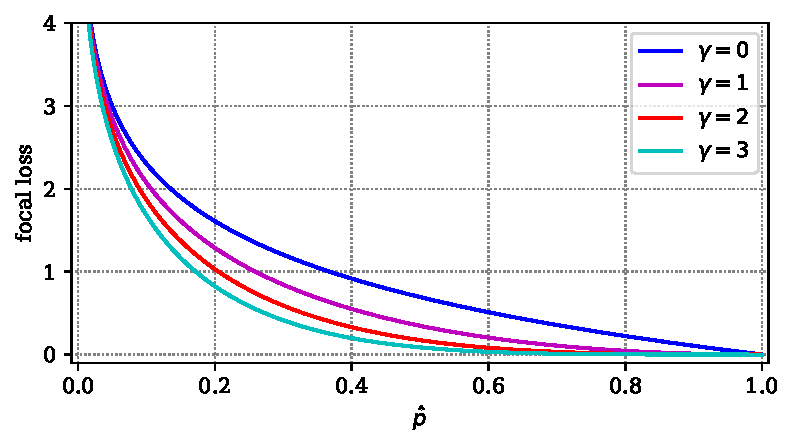
\includegraphics[width=0.7\textwidth]{focal_loss}
    \centering
    \caption{Фокальная ошибка для одного объекта. $\hat{p}$ --- оценка вероятности для истинного класса}
    \label{fig:focal_loss}
\end{figure}

Изначально фокальная ошибка была использована для устранения проблемы дисбаланса классов \cite{focal_detection}. С точки зрения калибровки уверенности идею впервые использовали в \cite{focal_calib}. Для объекта, принадлежащего $j$-му классу, фокальная ошибка имеет следующий вид:
\begin{equation}
    \operatorname{FL}=-(1-a_{j})^{\gamma}\cdot \log a_j, \quad \gamma \geqslant 0.
\end{equation}

При $\gamma=0$ функция потерь совпадает с кросс-энтропией. С увеличением $\gamma$, как видим на \autoref{fig:focal_loss}, уменьшается штраф за потери на объектах с уже высокой уверенностью в истинном классе. В то время как кросс-энтропия является верхней оценкой дивергенции Кульбака --- Лейблера между истинным $\vec{y}$ и предсказанным $\vec{a}$ распределением, у фокальной ошибки из оценки вычитается энтропия предсказанного распределения $H(\vec{a})$ \cite{focal_calib}:
\begin{equation*}
    \operatorname{CE}(\vec{y},\vec{a})
    \geqslant
    \operatorname{KL}(\vec{y}||\vec{a}),
    \qquad
    \operatorname{FL}(\vec{y},\vec{a})
    \geqslant
    \operatorname{KL}(\vec{y}||\vec{a})-\gamma\cdot \operatorname{H}(\vec{a}),
\end{equation*}
Получается, оптимизация фокальной ошибки дополнительно увеличивает энтропию предсказанного распределения, то есть помогает в борьбе с переуверенностью.

\section{Вычислительные эксперименты}\label{sec:experiments}

\subsection{Дизайн экспериментов}

В экспериментах были использованы следующие наборы данных:
\begin{itemize}
    \item \textbf{CIFAR-10} \cite{cifar}: Датасет содержит $60\,000$ цветных изображений $32\times 32$, каждое относится к одному из 10 классов. Разделение на \emph{обучающую} / \emph{валидационную} / \emph{тестовую} выборки: $50\,000\;/\;5\,000\;/\;5\,000$ изображений.
    \item \textbf{CIFAR-100} \cite{cifar}: $60\,000$ цветных изображений $32\times 32$, 100 классов. \emph{Обучение} / \emph{валидация} / \emph{тест}: $50\,000\;/\;5\,000\;/\;5\,000$.
    \item \textbf{ImageNet 2012} \cite{imagenet}: Крупный датасет с изображениями, разбитыми на 1000 классов. \emph{Обучение} / \emph{валидация} / \emph{тест}: $1.2\;\text{млн}\;/\;25\,000\;/\;25\,000$
    \item \textbf{Tiny ImageNet} \cite{imagenet}: $110\,000$ изображений $64\times 64$, разделенных на 200 классов. Является подмножеством предыдущего датасета. \emph{Обучение} / \emph{валидация} / \emph{тест}: $100\,000\;/\;5\,000\;/\;5\,000$.
\end{itemize}

Для вычислений использовались предобученные нейронные сети с различными архитектурами из открытых репозиториев. В экспериментах модели и датасеты разбиты на две основные группы:

\begin{enumerate}
    \item К первой группе отнесены нейронные сети, обученные на CIFAR-10, CIFAR-100, ImageNet. Веса для моделей были взяты соответственно из репозитериев \cite{pretrained_cifar10, pretrained_cifar100, pretrained_imagenet}. Модели данной группы используются для сравнения методов калибровки, основанных на постобработке.
    \item Ко второй группе отнесены предобученные нейросети из репозитория \cite{focal_github}. Здесь использованы датасеты CIFAR-10, CIFAR-100 и Tiny ImageNet. Данные нейросети были обучены для статьи \cite{focal_calib}~--- для части из них использовалась фокальная ошибка и сглаживание меток.
\end{enumerate}

При обучении модели настраивались на данные из \emph{обучающей} выборки (или ее части), калибровались на \emph{отложенной} выборке. Все построенные диаграммы надежности и метрики соответствуют \emph{тестовой} выборке.

Все эксперименты, реализация методов калибровки и оценок были выполнены на языке Python. Температурное, векторное и матричное шкалирование настраивались на GPU и были реализованы с использованием библиотеки PyTorch, остальные методы и метрики реализованы с использованием библиотек SciPy и sklearn. В гистограммном биннинге использовалось 20 бинов; ECE, cwECE и MCE считались для 15 бинов.

\subsection{Результаты}
Полные таблицы с измерениями приведены в 
\hyperref[sec:appendix]{приложении} к работе, диаграммы надежности для всех рассмотренных моделей можно найти в репозитории \cite{my_repo}.
\addrel{1}{21}{}

Рассмотрим диаграммы надежности для ShuffleNetV2 (CIFAR-100, \autoref{fig:reldiag_1_21}): можно видеть <<типичное>> состояние откалиброванности нейросети --- переуверенность. Калибровка помогает исправить ситуацию: в данном случае лучше с точки зрения всех метрик лучше всего сработало температурное шкалирование. Гистограммный бинниг работает слишком агрессивно для большого числа классов: в бинах часто оказывается мало объектов.

Для малого числа классов, напротив, гистограммный биннинг работает лучше всего с точки зрения уверенности в предсказании (\autoref{tab:metrics:ECE_1}, \autoref{tab:metrics:ECE_2} --- почти для всех моделей на CIFAR-10). Но отметим, что нейронные сети уже с очень высоким качеством решают такую задачу классификации. Почти все уверенности в предсказании близки к 1, как, например, на \autoref{fig:reldiag_2_1}. И с точки зрения MCE (\autoref{tab:metrics:MCE_1}, \autoref{tab:metrics:MCE_2}) --- метрики, в которой не учитываются <<веса>> бинов --- гистограммный биннинг дает низкое качество откалиброванности.
\addrel{2}{1}{}

Для матричного шкалирования мы не приводим диаграммы надежности: метод слишком сильно переобучается при большом числе классов. В итоге матричное шкалирование существенно ухудшает качество классификации (\autoref{tab:metrics:ACC_1}, \autoref{tab:metrics:ACC_1}) для всех датасетов, кроме, опять же, малоклассового CIFAR-10.

Одним из наиболее часто применяемых методов калибровки нейросетей является температурное шкалирование. Метод действительно не оказывает влияния на классификацию, в то время как другие варианты калибровки часто уменьшают точность (\autoref{tab:metrics:ACC_1}, \autoref{tab:metrics:ACC_2}). 

С точки зрения NLL ожидаемо лучшими оказались температурное и векторное шкалирование (ведь в процессе калибровки именно данная ошибки и оптимизировалась) --- \autoref{tab:metrics:NLL_1}, \autoref{tab:metrics:NLL_2}. Для Brier Score лучшим методом калибровки во многих случаях становилась изотоническая регрессия --- \autoref{tab:metrics:BS_1}, \autoref{tab:metrics:BS_2}. 

\begin{table}[h!]
    \begin{minipage}[h!]{0.47\textwidth}
        % \begin{table}[h!]
\centering
\resizebox{\textwidth}{!}{\begin{tabular}{lllllll}
\toprule
     Датасет &            Модель &    CE &  FL 1 &                  FL 2 &                  FL 3 &               LS 0.05 \\
\midrule
    CIFAR-10 &       DenseNet121 &  4.53 &  3.47 &                  2.02 &                  1.68 & \textbf{1.65} \\
    CIFAR-10 &         ResNet110 &  4.73 &  3.70 &                  2.78 & \textbf{1.61} &                  2.20 \\
    CIFAR-10 &          ResNet50 &  4.26 &  3.88 &                  2.55 & \textbf{1.58} &                  3.07 \\
    CIFAR-10 & Wide-ResNet-26-10 &  3.25 &  2.66 & \textbf{1.57} &                  1.98 &                  4.33 \\
   CIFAR-100 &       DenseNet121 & 20.90 & 14.54 &                  8.40 & \textbf{4.49} &                 13.27 \\
   CIFAR-100 &         ResNet110 & 19.76 & 15.35 &                 12.10 & \textbf{9.22} &                 11.44 \\
   CIFAR-100 &          ResNet50 & 18.14 & 13.36 &                  8.60 & \textbf{4.99} &                  8.15 \\
   CIFAR-100 & Wide-ResNet-26-10 & 16.28 &  9.12 &                  4.22 & \textbf{2.20} &                  5.27 \\
TinyImageNet &          ResNet50 & 15.98 &  7.87 &                  3.32 & \textbf{1.93} &                 15.73 \\
\bottomrule
\end{tabular}%
}
\caption{ECE, \% -- Expected Calibration Error, (меньше -- лучше), 15 бинов без постобработки, столбцы соответствуют разным функциям потерь}
\label{tab:fl:ECE}
% \end{table}

    \end{minipage}\hfill
    \begin{minipage}[h!]{0.47\textwidth}
        % \begin{table}[h!]
\centering
\resizebox{\textwidth}{!}{\begin{tabular}{lllllll}
\toprule
     Датасет &            Модель &    CE &  FL 1 &                   FL 2 &                   FL 3 & LS 0.05 \\
\midrule
    CIFAR-10 &       DenseNet121 & 0.948 & 0.755 & \textbf{0.514} &                  0.524 &   0.576 \\
    CIFAR-10 &         ResNet110 & 0.990 & 0.804 &                  0.660 & \textbf{0.505} &   0.673 \\
    CIFAR-10 &          ResNet50 & 0.941 & 0.836 &                  0.625 & \textbf{0.524} &   0.766 \\
    CIFAR-10 & Wide-ResNet-26-10 & 0.699 & 0.611 & \textbf{0.479} &                  0.523 &   0.869 \\
   CIFAR-100 &       DenseNet121 & 0.458 & 0.364 &                  0.280 & \textbf{0.254} &   0.315 \\
   CIFAR-100 &         ResNet110 & 0.433 & 0.372 &                  0.321 & \textbf{0.281} &   0.299 \\
   CIFAR-100 &          ResNet50 & 0.412 & 0.337 &                  0.282 & \textbf{0.256} &   0.271 \\
   CIFAR-100 & Wide-ResNet-26-10 & 0.372 & 0.264 & \textbf{0.218} &                  0.226 &   0.239 \\
TinyImageNet &          ResNet50 & 0.250 & 0.218 &                  0.205 & \textbf{0.203} &   0.231 \\
\bottomrule
\end{tabular}%
}
\caption{cwECE, \% -- Classwise Expected Calibration Error (меньше -- лучше), 15 бинов без постобработки, столбцы соответствуют разным функциям потерь}
\label{tab:fl:cwECE}
% \end{table}

    \end{minipage}
\end{table}
\addrel{1}{29}{}
Фокальная ошибка и сглаживание меток действительно дают более откалибровнные модели, чем при настройке на стандартную кросс-энтропию — как с точки уверенности в предсказанном класса (\autoref{tab:fl:ECE}), так и с точки зрения поклассовых оценок (\autoref{tab:fl:cwECE}). При этом далее модели можно калибровать с помощью постобработки. В оригинальной работе \cite{focal_calib} для калибровки моделей, обученных на фокальную ошибку, использовалось только температурное шкалирование. Хотя относительно ECE (\autoref{tab:metrics:ECE_2}) такой подход действительно показывает высокие результаты, для поклассовой cwECE (\autoref{tab:metrics:cwECE_2}) чаще лучше работает векторное шкалирование. Для моделей первой группы (\autoref{tab:metrics:cwECE_1}) векторное шкалирование тоже в основном минимизирует cwECE. Такие результаты вполне ожидаемы, поскольку векторное шкалирование находит отдельные коэффициенты деформации для каждого класса.

Рассмотрим также диаграммы калибровки для EfficientNet (\autoref{fig:reldiag_1_29}). Среди всех использованных моделей, у данной нейросети четче всего видна недоуверенность --- большая часть оценок сосредоточена не на $[0.9, 1]$, а на $[0.8, 0.9)$. Причина такого поведения может быть как раз в особенности обучения: модель обучалась со сглаживанием меток ($\alpha=0.1$) \cite{pretrained_imagenet}. Все методы калибровки привели к заметному повышению уверенности.


\section{Заключение}
Таким образом, в данной работе мы сравнили основные методы калибровки, эксперименты были проведены для различных архитектур сверточных нейросетей. Применимость того или иного алгоритма калибровки существенно зависит от количества данных и выбранного критерия качества. Методы, строящие отдельные функции деформации для каждого класса, показывают высокое качество только при достаточном размере отложенной выборке (соответственно, небольшом числе классов). Стратегии, в основе которых лежит линейное преобразование логитов (например, температурное шкалирование) лучше работают для задач с большим числом классов, но сильно переобучаются при чрезмерной параметризации (матричное шкалирование). Калибровка уверенности до сих пор остается открытой проблемой, и даже способ оценки откалиброванности модели не является решенным вопросом. 

\newpage
% \section{Список литературы}
\printbibliography[
    heading=bibintoc,
    title={Список литературы}
]

\newpage
\begin{appendices}\label{sec:appendix}
\section{Качество классификации моделей}
\begin{table}[h!]
\centering
\resizebox{\textwidth}{!}{\begin{tabular}{llccccccc}
\toprule
  Датасет &            Модель &          До калибровки &           Hist-binning &               Isotonic &              T-scaling &              V-scaling &            V-scaling-b &            M-scaling-b \\
\midrule
 CIFAR-10 &       DenseNet121 & \textbf{93.92} &                  93.52 &                  93.72 & \textbf{93.92} &                  93.84 &                  93.80 &                  93.80 \\
 CIFAR-10 &       DenseNet161 &                  93.70 & \textbf{93.74} &                  93.58 &                  93.70 &                  93.72 & \textbf{93.74} &                  93.52 \\
 CIFAR-10 &       DenseNet169 & \textbf{94.08} &                  93.44 &                  93.84 & \textbf{94.08} &                  94.02 &                  93.94 &                  93.78 \\
 CIFAR-10 &         GoogleNet & \textbf{92.92} &                  92.58 &                  92.68 & \textbf{92.92} &                  92.90 &                  92.84 &                  92.76 \\
 CIFAR-10 &       InceptionV3 & \textbf{93.32} &                  93.12 &                  93.28 & \textbf{93.32} &                  93.22 & \textbf{93.32} &                  93.26 \\
 CIFAR-10 &       MobileNetV2 & \textbf{93.42} &                  93.40 & \textbf{93.42} & \textbf{93.42} &                  93.26 &                  93.36 &                  93.36 \\
 CIFAR-10 &          ResNet18 & \textbf{92.54} &                  92.14 &                  92.34 & \textbf{92.54} &                  92.48 &                  92.40 &                  92.18 \\
 CIFAR-10 &          ResNet34 & \textbf{93.24} &                  92.74 &                  92.92 & \textbf{93.24} &                  93.14 &                  93.16 &                  92.94 \\
 CIFAR-10 &          ResNet50 & \textbf{93.44} &                  93.10 &                  93.22 & \textbf{93.44} &                  93.40 &                  93.38 &                  93.24 \\
 CIFAR-10 &          VGG11\_bn &                  91.96 &                  91.66 &                  91.84 &                  91.96 &                  91.86 &                  91.80 & \textbf{91.98} \\
 CIFAR-10 &          VGG13\_bn &                  93.86 &                  93.40 &                  93.74 &                  93.86 & \textbf{93.92} &                  93.82 &                  93.68 \\
 CIFAR-10 &          VGG16\_bn & \textbf{93.52} &                  93.38 &                  93.42 & \textbf{93.52} &                  93.36 &                  93.36 &                  93.36 \\
 CIFAR-10 &          VGG19\_bn &                  93.76 &                  93.36 &                  93.62 &                  93.76 &                  93.70 & \textbf{93.84} &                  93.56 \\
CIFAR-100 &  MobileNetV2\_x0\_5 & \textbf{70.32} &                  67.56 &                  69.86 & \textbf{70.32} &                  70.26 &                  69.94 &                  55.38 \\
CIFAR-100 &  MobileNetV2\_x1\_0 &                  73.34 &                  70.74 &                  72.98 &                  73.34 &                  73.20 & \textbf{73.50} &                  59.24 \\
CIFAR-100 &  MobileNetV2\_x1\_4 & \textbf{76.22} &                  72.96 &                  75.58 & \textbf{76.22} &                  75.72 &                  75.80 &                  63.10 \\
CIFAR-100 &          ResNet20 & \textbf{67.80} &                  63.80 &                  66.72 & \textbf{67.80} &                  67.36 &                  67.54 &                  49.94 \\
CIFAR-100 &          ResNet32 & \textbf{69.10} &                  65.90 &                  68.64 & \textbf{69.10} &                  68.90 &                  68.70 &                  52.20 \\
CIFAR-100 &          ResNet44 & \textbf{70.82} &                  67.86 &                  70.22 & \textbf{70.82} &                  70.42 &                  70.56 &                  55.16 \\
CIFAR-100 &          ResNet56 & \textbf{72.04} &                  69.54 &                  71.62 & \textbf{72.04} &                  71.72 &                  71.58 &                  56.34 \\
CIFAR-100 & ShuffleNetV2\_x0\_5 &                  66.86 &                  64.22 &                  66.68 &                  66.86 & \textbf{66.98} &                  66.58 &                  50.02 \\
CIFAR-100 & ShuffleNetV2\_x1\_0 & \textbf{71.58} &                  69.16 &                  71.24 & \textbf{71.58} &                  71.26 &                  71.30 &                  57.50 \\
CIFAR-100 & ShuffleNetV2\_x1\_5 &                  73.60 &                  70.90 &                  73.34 &                  73.60 &                  73.72 & \textbf{73.80} &                  61.30 \\
CIFAR-100 & ShuffleNetV2\_x2\_0 & \textbf{74.92} &                  72.30 &                  74.44 & \textbf{74.92} &                  74.84 &                  74.82 &                  63.04 \\
CIFAR-100 &          VGG11\_bn & \textbf{69.96} &                  67.76 &                  69.34 & \textbf{69.96} &                  69.56 &                  69.58 &                  59.90 \\
CIFAR-100 &          VGG13\_bn & \textbf{73.90} &                  71.84 &                  73.02 & \textbf{73.90} &                  73.56 &                  73.36 &                  62.58 \\
CIFAR-100 &          VGG16\_bn & \textbf{73.30} &                  71.34 &                  72.78 & \textbf{73.30} &                  72.96 &                  72.94 &                  64.28 \\
CIFAR-100 &          VGG19\_bn & \textbf{73.14} &                  71.78 &                  72.76 & \textbf{73.14} &                  73.00 &                  72.82 &                  63.78 \\
 ImageNet &   EfficientNet\_b8 &                  85.52 &                  83.43 &                  84.92 &                  85.52 & \textbf{85.54} &                  85.47 &                  79.12 \\
 ImageNet &  MobileNetV2\_120d & \textbf{77.68} &                  73.57 &                  76.79 & \textbf{77.68} &                  77.36 &                  77.16 &                  59.84 \\
 ImageNet &         RepVGG\_b3 & \textbf{80.57} &                  77.68 &                  79.89 & \textbf{80.57} &                  80.22 &                  80.17 &                  66.38 \\
 ImageNet &          VGG19\_bn & \textbf{74.35} &                  70.47 &                  73.72 & \textbf{74.35} &                  73.92 &                  73.62 &                  54.06 \\
\bottomrule
\end{tabular}%
}
\caption{Accuracy, \% (больше -- лучше) -- доля правильных ответов, группа 1}
\label{tab:metrics:ACC_1}
\end{table}

\begin{table}[h!]
\centering
\resizebox{\textwidth}{!}{\begin{tabular}{llccccccc}
\toprule
     Датасет &                      Модель &          До калибровки &           Hist-binning &               Isotonic &              T-scaling &              V-scaling &            V-scaling-b &            M-scaling-b \\
\midrule
    CIFAR-10 &            DenseNet121 (CE) &                  94.92 & \textbf{94.98} &                  94.84 &                  94.92 &                  94.94 &                  94.96 &                  94.76 \\
    CIFAR-10 &          DenseNet121 (FL 1) &                  94.84 &                  94.68 &                  94.82 &                  94.84 &                  95.00 & \textbf{95.02} &                  94.52 \\
    CIFAR-10 &          DenseNet121 (FL 2) &                  94.90 &                  94.60 & \textbf{94.96} &                  94.90 &                  94.84 &                  94.80 &                  94.80 \\
    CIFAR-10 &          DenseNet121 (FL 3) &                  94.24 &                  94.24 &                  94.20 &                  94.24 &                  94.34 &                  94.24 & \textbf{94.36} \\
    CIFAR-10 &       DenseNet121 (LS 0.05) &                  94.52 &                  94.62 & \textbf{94.66} &                  94.52 &                  94.56 &                  94.58 &                  94.62 \\
    CIFAR-10 &              ResNet110 (CE) &                  94.82 &                  94.70 &                  94.76 &                  94.82 &                  94.84 &                  94.86 & \textbf{94.90} \\
    CIFAR-10 &            ResNet110 (FL 1) &                  94.80 &                  94.90 &                  94.84 &                  94.80 &                  94.86 & \textbf{95.00} &                  94.98 \\
    CIFAR-10 &            ResNet110 (FL 2) &                  94.82 &                  94.82 & \textbf{94.96} &                  94.82 & \textbf{94.96} &                  94.90 &                  94.84 \\
    CIFAR-10 &            ResNet110 (FL 3) &                  94.70 &                  94.64 &                  94.84 &                  94.70 &                  94.84 & \textbf{94.86} &                  94.70 \\
    CIFAR-10 &         ResNet110 (LS 0.05) &                  94.36 &                  94.36 & \textbf{94.48} &                  94.36 &                  94.32 &                  94.32 &                  94.40 \\
    CIFAR-10 &               ResNet50 (CE) & \textbf{95.02} &                  94.62 &                  94.66 & \textbf{95.02} &                  95.00 &                  94.96 &                  94.82 \\
    CIFAR-10 &             ResNet50 (FL 1) &                  94.58 &                  94.34 &                  94.52 &                  94.58 & \textbf{94.60} &                  94.52 &                  94.58 \\
    CIFAR-10 &             ResNet50 (FL 2) &                  94.80 &                  94.62 &                  94.82 &                  94.80 & \textbf{94.90} & \textbf{94.90} &                  94.88 \\
    CIFAR-10 &             ResNet50 (FL 3) &                  94.52 &                  94.48 & \textbf{94.66} &                  94.52 &                  94.58 &                  94.60 &                  94.44 \\
    CIFAR-10 &          ResNet50 (LS 0.05) &                  94.26 &                  94.02 &                  94.18 &                  94.26 &                  94.26 &                  94.16 & \textbf{94.30} \\
    CIFAR-10 &      Wide-ResNet-26-10 (CE) &                  96.12 &                  96.02 &                  96.08 &                  96.12 & \textbf{96.20} & \textbf{96.20} &                  96.10 \\
    CIFAR-10 &    Wide-ResNet-26-10 (FL 1) & \textbf{95.70} &                  95.26 &                  95.56 & \textbf{95.70} &                  95.64 &                  95.66 & \textbf{95.70} \\
    CIFAR-10 &    Wide-ResNet-26-10 (FL 2) & \textbf{95.56} &                  95.06 &                  95.50 & \textbf{95.56} &                  95.40 &                  95.46 &                  95.48 \\
    CIFAR-10 &    Wide-ResNet-26-10 (FL 3) &                  95.64 &                  95.62 & \textbf{95.80} &                  95.64 &                  95.74 &                  95.74 &                  95.64 \\
    CIFAR-10 & Wide-ResNet-26-10 (LS 0.05) &                  95.66 &                  95.50 &                  95.40 &                  95.66 &                  95.64 & \textbf{95.68} &                  95.42 \\
   CIFAR-100 &            DenseNet121 (CE) &                  75.32 &                  74.52 &                  75.26 &                  75.32 & \textbf{75.76} &                  75.70 &                  65.60 \\
   CIFAR-100 &          DenseNet121 (FL 1) &                  75.66 &                  74.12 &                  75.90 &                  75.66 & \textbf{76.02} &                  76.00 &                  65.24 \\
   CIFAR-100 &          DenseNet121 (FL 2) &                  75.90 &                  73.50 & \textbf{76.22} &                  75.90 &                  75.90 &                  76.02 &                  65.32 \\
   CIFAR-100 &          DenseNet121 (FL 3) &                  76.10 &                  72.90 &                  75.86 &                  76.10 &                  76.16 & \textbf{76.20} &                  65.06 \\
   CIFAR-100 &       DenseNet121 (LS 0.05) &                  75.54 &                  74.56 &                  75.66 &                  75.54 &                  75.66 & \textbf{75.74} &                  66.60 \\
   CIFAR-100 &              ResNet110 (CE) &                  76.44 &                  76.02 &                  76.50 &                  76.44 &                  76.80 & \textbf{76.88} &                  66.20 \\
   CIFAR-100 &            ResNet110 (FL 1) &                  76.84 &                  75.28 &                  76.48 &                  76.84 & \textbf{77.34} &                  77.28 &                  66.52 \\
   CIFAR-100 &            ResNet110 (FL 2) &                  76.74 &                  74.48 &                  76.68 &                  76.74 & \textbf{77.04} &                  76.90 &                  67.00 \\
   CIFAR-100 &            ResNet110 (FL 3) &                  76.30 &                  74.80 &                  76.56 &                  76.30 &                  76.66 & \textbf{76.82} &                  66.46 \\
   CIFAR-100 &         ResNet110 (LS 0.05) &                  75.96 &                  74.48 &                  75.68 &                  75.96 &                  76.10 & \textbf{76.18} &                  66.66 \\
   CIFAR-100 &               ResNet50 (CE) &                  76.00 &                  74.48 &                  75.62 &                  76.00 &                  76.12 & \textbf{76.14} &                  65.86 \\
   CIFAR-100 &             ResNet50 (FL 1) &                  76.38 &                  74.22 &                  76.36 &                  76.38 & \textbf{76.66} &                  76.46 &                  66.32 \\
   CIFAR-100 &             ResNet50 (FL 2) & \textbf{76.58} &                  73.90 &                  76.10 & \textbf{76.58} &                  76.52 &                  76.46 &                  65.40 \\
   CIFAR-100 &             ResNet50 (FL 3) & \textbf{77.08} &                  74.44 &                  76.42 & \textbf{77.08} &                  76.86 &                  76.94 &                  64.62 \\
   CIFAR-100 &          ResNet50 (LS 0.05) &                  76.18 &                  74.38 &                  76.24 &                  76.18 &                  76.42 & \textbf{76.48} &                  67.98 \\
   CIFAR-100 &      Wide-ResNet-26-10 (CE) &                  78.26 &                  77.22 &                  77.98 &                  78.26 & \textbf{78.38} &                  78.22 &                  67.72 \\
   CIFAR-100 &    Wide-ResNet-26-10 (FL 1) & \textbf{79.84} &                  78.10 &                  79.80 & \textbf{79.84} &                  79.76 &                  79.76 &                  68.82 \\
   CIFAR-100 &    Wide-ResNet-26-10 (FL 2) &                  79.64 &                  77.54 &                  79.64 &                  79.64 &                  79.96 & \textbf{80.04} &                  69.44 \\
   CIFAR-100 &    Wide-ResNet-26-10 (FL 3) &                  79.70 &                  76.96 &                  79.62 &                  79.70 & \textbf{79.86} &                  79.80 &                  70.18 \\
   CIFAR-100 & Wide-ResNet-26-10 (LS 0.05) &                  78.14 &                  75.98 &                  77.90 &                  78.14 & \textbf{78.26} &                  78.24 &                  69.62 \\
TinyImageNet &               ResNet50 (CE) & \textbf{49.98} &                  44.92 &                  49.10 & \textbf{49.98} &                  49.44 &                  49.24 &                  32.66 \\
TinyImageNet &             ResNet50 (FL 1) & \textbf{50.10} &                  44.96 &                  49.48 & \textbf{50.10} &                  50.04 &                  49.94 &                  31.32 \\
TinyImageNet &             ResNet50 (FL 2) & \textbf{51.86} &                  46.56 &                  51.14 & \textbf{51.86} &                  51.82 &                  51.62 &                  31.96 \\
TinyImageNet &             ResNet50 (FL 3) & \textbf{51.06} &                  44.56 &                  50.18 & \textbf{51.06} &                  50.82 &                  50.94 &                  32.08 \\
TinyImageNet &          ResNet50 (LS 0.05) & \textbf{53.62} &                  47.18 &                  51.94 & \textbf{53.62} &                  52.84 &                  52.78 &                  36.82 \\
\bottomrule
\end{tabular}%
}
\caption{Accuracy, \% (больше -- лучше) -- доля правильных ответов, группа 2}
\label{tab:metrics:ACC_2}
\end{table}

\clearpage

\section{Биннинговые метрики}
\begin{table}[h!]
\centering
\resizebox{\textwidth}{!}{\begin{tabular}{llccccccc}
\toprule
  Датасет &            Модель &         До калибровки &          Hist-binning &              Isotonic &             T-scaling &             V-scaling &           V-scaling-b & M-scaling-b \\
\midrule
 CIFAR-10 &       DenseNet121 &                  1.86 & \textbf{1.08} &                  2.10 &                  1.64 &                  1.67 &                  1.58 &        1.49 \\
 CIFAR-10 &       DenseNet161 &                  2.11 & \textbf{1.08} &                  1.64 &                  1.68 &                  1.87 &                  1.75 &        1.75 \\
 CIFAR-10 &       DenseNet169 &                  2.04 & \textbf{1.42} &                  1.87 &                  1.72 &                  1.64 &                  1.62 &        1.64 \\
 CIFAR-10 &         GoogleNet &                  1.65 & \textbf{0.89} &                  1.36 &                  1.21 &                  1.46 &                  1.37 &        1.34 \\
 CIFAR-10 &       InceptionV3 &                  2.06 & \textbf{1.35} &                  1.91 &                  1.88 &                  1.99 &                  1.91 &        1.86 \\
 CIFAR-10 &       MobileNetV2 &                  2.92 & \textbf{1.45} &                  1.74 &                  1.87 &                  2.09 &                  1.95 &        1.78 \\
 CIFAR-10 &          ResNet18 &                  2.51 & \textbf{1.60} &                  2.03 &                  2.13 &                  1.98 &                  1.93 &        2.16 \\
 CIFAR-10 &          ResNet34 &                  2.67 & \textbf{1.44} &                  2.09 &                  1.96 &                  1.70 &                  1.88 &        1.75 \\
 CIFAR-10 &          ResNet50 &                  2.50 & \textbf{1.06} &                  1.70 &                  1.67 &                  1.72 &                  1.59 &        1.62 \\
 CIFAR-10 &          VGG11\_bn &                  1.87 &                  2.21 & \textbf{1.65} &                  1.83 &                  1.88 &                  1.90 &        1.76 \\
 CIFAR-10 &          VGG13\_bn & \textbf{1.41} &                  1.42 &                  1.54 &                  1.44 &                  1.44 &                  1.43 &        1.72 \\
 CIFAR-10 &          VGG16\_bn &                  1.86 & \textbf{1.08} &                  1.61 &                  1.71 &                  1.93 &                  1.81 &        1.74 \\
 CIFAR-10 &          VGG19\_bn &                  2.15 & \textbf{1.02} &                  1.34 &                  1.87 &                  2.00 &                  1.98 &        2.14 \\
CIFAR-100 &  MobileNetV2\_x0\_5 &                 12.69 &                  9.39 &                  5.86 & \textbf{3.28} &                  3.31 &                  3.57 &       44.57 \\
CIFAR-100 &  MobileNetV2\_x1\_0 &                 11.77 &                 10.13 &                  6.02 &                  3.78 & \textbf{3.46} &                  3.69 &       40.68 \\
CIFAR-100 &  MobileNetV2\_x1\_4 &                  9.66 &                 10.13 &                  4.29 &                  2.90 & \textbf{2.69} &                  2.86 &       36.79 \\
CIFAR-100 &          ResNet20 &                 11.21 &                  9.01 &                  5.79 & \textbf{2.48} &                  3.11 &                  3.13 &       50.05 \\
CIFAR-100 &          ResNet32 &                 13.95 &                 10.34 &                  5.47 &                  2.61 & \textbf{2.28} &                  2.77 &       47.79 \\
CIFAR-100 &          ResNet44 &                 14.99 &                  8.42 &                  6.42 & \textbf{3.18} &                  3.49 &                  3.48 &       44.84 \\
CIFAR-100 &          ResNet56 &                 14.72 &                  7.86 &                  5.68 &                  3.13 & \textbf{3.10} &                  3.40 &       43.65 \\
CIFAR-100 & ShuffleNetV2\_x0\_5 &                 12.93 &                  9.62 &                  5.38 & \textbf{2.22} &                  2.38 &                  2.80 &       49.77 \\
CIFAR-100 & ShuffleNetV2\_x1\_0 &                 11.68 &                  8.15 &                  5.90 & \textbf{3.68} &                  4.24 &                  4.18 &       42.32 \\
CIFAR-100 & ShuffleNetV2\_x1\_5 &                  9.86 &                  8.94 &                  5.44 & \textbf{4.56} &                  4.88 &                  4.64 &       38.44 \\
CIFAR-100 & ShuffleNetV2\_x2\_0 &                  7.68 &                 10.14 &                  4.91 & \textbf{4.26} &                  4.78 &                  4.78 &       36.80 \\
CIFAR-100 &          VGG11\_bn &                 15.86 &                 10.61 &                  7.78 & \textbf{5.17} &                  5.80 &                  6.08 &       29.38 \\
CIFAR-100 &          VGG13\_bn &                 14.06 &                  8.12 &                  7.19 &                  5.84 & \textbf{5.80} &                  5.84 &       27.53 \\
CIFAR-100 &          VGG16\_bn &                 19.33 &                  8.87 &                  5.74 &                  4.18 & \textbf{3.93} &                  4.03 &       28.60 \\
CIFAR-100 &          VGG19\_bn &                 20.17 &                  8.79 &                  5.22 &                  4.53 &                  3.74 & \textbf{3.61} &       31.98 \\
 ImageNet &   EfficientNet\_b8 &                  8.98 &                  4.88 & \textbf{2.96} &                  3.17 &                  3.51 &                  3.95 &       20.15 \\
 ImageNet &  MobileNetV2\_120d &                  6.85 &                  7.02 &                  1.96 & \textbf{1.61} &                  2.11 &                  2.90 &       38.18 \\
 ImageNet &         RepVGG\_b3 & \textbf{3.23} &                  6.17 &                  3.61 &                  3.95 &                  4.08 &                  4.76 &       32.42 \\
 ImageNet &          VGG19\_bn &                  3.69 &                  9.26 &                  3.93 &                  1.92 & \textbf{1.53} &                  2.16 &       44.68 \\
\bottomrule
\end{tabular}%
}
\caption{ECE, \% -- Expected Calibration Error, (меньше -- лучше), 15 бинов группа 1}
\label{tab:metrics:ECE_1}
\end{table}

\begin{table}[h!]
\centering
\resizebox{\textwidth}{!}{\begin{tabular}{llccccccc}
\toprule
     Датасет &                      Модель &         До калибровки &          Hist-binning &              Isotonic &             T-scaling &             V-scaling &           V-scaling-b &           M-scaling-b \\
\midrule
    CIFAR-10 &            DenseNet121 (CE) &                  4.53 & \textbf{0.38} &                  1.24 &                  1.64 &                  1.19 &                  1.29 &                  1.45 \\
    CIFAR-10 &          DenseNet121 (FL 1) &                  3.47 &                  0.87 & \textbf{0.65} &                  1.26 &                  0.88 &                  1.05 &                  1.44 \\
    CIFAR-10 &          DenseNet121 (FL 2) &                  2.02 &                  0.97 & \textbf{0.73} &                  0.95 &                  1.08 &                  1.01 &                  1.18 \\
    CIFAR-10 &          DenseNet121 (FL 3) &                  1.68 & \textbf{1.17} &                  1.32 &                  1.49 &                  1.32 &                  1.38 &                  1.84 \\
    CIFAR-10 &       DenseNet121 (LS 0.05) &                  1.65 & \textbf{0.93} &                  1.55 &                  1.22 &                  1.28 &                  1.24 &                  1.29 \\
    CIFAR-10 &              ResNet110 (CE) &                  4.73 & \textbf{1.01} &                  1.11 &                  1.23 &                  1.36 &                  1.39 &                  1.25 \\
    CIFAR-10 &            ResNet110 (FL 1) &                  3.70 & \textbf{0.71} &                  0.99 &                  1.11 &                  1.20 &                  1.06 &                  1.05 \\
    CIFAR-10 &            ResNet110 (FL 2) &                  2.78 & \textbf{0.55} &                  1.20 &                  1.03 &                  0.94 &                  0.96 &                  1.07 \\
    CIFAR-10 &            ResNet110 (FL 3) &                  1.61 & \textbf{0.84} &                  0.96 &                  1.24 &                  0.94 &                  0.84 &                  1.01 \\
    CIFAR-10 &         ResNet110 (LS 0.05) &                  2.20 &                  1.77 &                  0.90 &                  1.56 &                  1.07 &                  0.88 & \textbf{0.72} \\
    CIFAR-10 &               ResNet50 (CE) &                  4.26 & \textbf{0.70} &                  0.96 &                  1.41 &                  1.17 &                  1.10 &                  1.23 \\
    CIFAR-10 &             ResNet50 (FL 1) &                  3.88 &                  1.88 & \textbf{1.46} &                  1.58 &                  1.65 &                  1.67 &                  1.85 \\
    CIFAR-10 &             ResNet50 (FL 2) &                  2.55 & \textbf{1.08} &                  1.09 &                  1.17 &                  1.52 &                  1.52 &                  1.14 \\
    CIFAR-10 &             ResNet50 (FL 3) &                  1.58 & \textbf{0.78} &                  0.98 &                  1.11 &                  1.16 &                  1.01 &                  1.56 \\
    CIFAR-10 &          ResNet50 (LS 0.05) &                  3.07 &                  1.23 & \textbf{1.14} &                  1.35 &                  1.35 &                  1.43 &                  1.40 \\
    CIFAR-10 &      Wide-ResNet-26-10 (CE) &                  3.25 &                  0.60 & \textbf{0.50} &                  1.07 &                  0.84 &                  0.91 &                  0.90 \\
    CIFAR-10 &    Wide-ResNet-26-10 (FL 1) &                  2.66 &                  0.95 &                  1.03 & \textbf{0.87} &                  1.08 &                  1.17 &                  1.05 \\
    CIFAR-10 &    Wide-ResNet-26-10 (FL 2) &                  1.57 &                  1.40 & \textbf{1.12} &                  1.18 &                  1.37 &                  1.31 &                  1.42 \\
    CIFAR-10 &    Wide-ResNet-26-10 (FL 3) &                  1.98 & \textbf{0.82} &                  0.89 &                  1.06 &                  1.08 &                  0.86 &                  0.89 \\
    CIFAR-10 & Wide-ResNet-26-10 (LS 0.05) &                  4.33 & \textbf{0.72} &                  0.94 &                  0.99 &                  1.17 &                  1.17 &                  1.23 \\
   CIFAR-100 &            DenseNet121 (CE) &                 20.90 &                  7.00 &                  6.18 &                  4.82 &                  4.74 & \textbf{4.72} &                 34.38 \\
   CIFAR-100 &          DenseNet121 (FL 1) &                 14.54 &                  6.03 &                  7.31 & \textbf{5.18} &                  5.22 &                  5.38 &                 34.71 \\
   CIFAR-100 &          DenseNet121 (FL 2) &                  8.40 &                 10.42 &                  4.47 & \textbf{4.16} &                  4.37 &                  4.42 &                 34.63 \\
   CIFAR-100 &          DenseNet121 (FL 3) &                  4.49 &                  9.10 &                  4.16 & \textbf{3.98} &                  4.55 &                  4.45 &                 34.84 \\
   CIFAR-100 &       DenseNet121 (LS 0.05) &                 13.27 &                  6.98 &                  7.03 &                  7.44 & \textbf{3.32} &                  3.49 &                 33.31 \\
   CIFAR-100 &              ResNet110 (CE) &                 19.76 & \textbf{3.99} &                  6.09 &                  5.63 &                  5.37 &                  5.44 &                 33.74 \\
   CIFAR-100 &            ResNet110 (FL 1) &                 15.35 &                  6.16 &                  6.56 &                  4.87 & \textbf{4.83} &                  4.84 &                 33.41 \\
   CIFAR-100 &            ResNet110 (FL 2) &                 12.10 &                  8.50 &                  5.92 & \textbf{5.48} &                  5.51 &                  5.61 &                 32.91 \\
   CIFAR-100 &            ResNet110 (FL 3) &                  9.22 &                  8.68 & \textbf{4.67} &                  5.36 &                  5.41 &                  5.39 &                 33.53 \\
   CIFAR-100 &         ResNet110 (LS 0.05) &                 11.44 &                  6.95 &                  5.86 & \textbf{4.41} &                  4.50 &                  4.66 &                 33.25 \\
   CIFAR-100 &               ResNet50 (CE) &                 18.14 & \textbf{4.75} &                  7.24 &                  6.02 &                  6.52 &                  6.53 &                 34.07 \\
   CIFAR-100 &             ResNet50 (FL 1) &                 13.36 &                  5.81 &                  7.06 & \textbf{5.29} &                  5.44 &                  5.61 &                 33.62 \\
   CIFAR-100 &             ResNet50 (FL 2) &                  8.60 &                  9.41 &                  4.90 & \textbf{4.72} &                  4.91 &                  4.90 &                 34.52 \\
   CIFAR-100 &             ResNet50 (FL 3) &                  4.99 &                  7.73 &                  4.07 & \textbf{3.39} &                  3.83 &                  3.98 &                 35.30 \\
   CIFAR-100 &          ResNet50 (LS 0.05) &                  8.15 &                  7.68 &                  6.61 & \textbf{5.27} &                  5.32 &                  5.32 &                 31.94 \\
   CIFAR-100 &      Wide-ResNet-26-10 (CE) &                 16.28 &                  4.91 &                  6.43 & \textbf{4.79} &                  5.21 &                  5.00 &                 32.23 \\
   CIFAR-100 &    Wide-ResNet-26-10 (FL 1) &                  9.12 &                  8.12 &                  5.40 &                  4.31 &                  4.35 & \textbf{4.24} &                 31.16 \\
   CIFAR-100 &    Wide-ResNet-26-10 (FL 2) &                  4.22 &                  7.61 & \textbf{3.47} &                  3.87 &                  4.01 &                  3.75 &                 30.53 \\
   CIFAR-100 &    Wide-ResNet-26-10 (FL 3) & \textbf{2.20} &                  8.05 &                  3.33 &                  3.62 &                  3.62 &                  3.79 &                 29.80 \\
   CIFAR-100 & Wide-ResNet-26-10 (LS 0.05) &                  5.27 &                  7.52 &                  5.36 & \textbf{4.78} &                  4.85 &                  4.83 &                 30.37 \\
TinyImageNet &               ResNet50 (CE) &                 15.98 &                  9.96 &                 10.06 & \textbf{6.67} &                  7.26 &                  7.83 &                 65.77 \\
TinyImageNet &             ResNet50 (FL 1) &                  7.87 &                  9.96 &                  6.12 & \textbf{4.17} &                  4.76 &                  5.54 &                 67.23 \\
TinyImageNet &             ResNet50 (FL 2) &                  3.32 &                  9.49 &                  4.94 & \textbf{2.98} &                  3.63 &                  3.82 &                 66.81 \\
TinyImageNet &             ResNet50 (FL 3) &                  1.93 &                  9.88 &                  3.13 & \textbf{1.77} &                  2.61 &                  2.70 &                 66.65 \\
TinyImageNet &          ResNet50 (LS 0.05) &                 15.73 &                  6.29 & \textbf{3.02} &                  7.02 &                  7.18 &                  7.56 &                 60.64 \\
\bottomrule
\end{tabular}%
}
\caption{ECE, \% -- Expected Calibration Error, (меньше -- лучше), 15 бинов группа 2}
\label{tab:metrics:ECE_2}
\end{table}

\begin{table}[h!]
\centering
\resizebox{\textwidth}{!}{\begin{tabular}{llccccccc}
\toprule
  Датасет &            Модель & До калибровки &           Hist-binning &               Isotonic &              T-scaling &              V-scaling &            V-scaling-b &            M-scaling-b \\
\midrule
 CIFAR-10 &       DenseNet121 &         0.513 &                  0.509 &                  0.566 &                  0.514 &                  0.548 &                  0.491 & \textbf{0.483} \\
 CIFAR-10 &       DenseNet161 &         0.646 &                  0.536 &                  0.534 &                  0.629 &                  0.531 & \textbf{0.527} &                  0.536 \\
 CIFAR-10 &       DenseNet169 &         0.551 &                  0.566 &                  0.527 &                  0.536 & \textbf{0.485} &                  0.490 &                  0.518 \\
 CIFAR-10 &         GoogleNet &         0.641 &                  0.579 &                  0.543 &                  0.559 &                  0.544 & \textbf{0.520} &                  0.545 \\
 CIFAR-10 &       InceptionV3 &         0.596 &                  0.573 & \textbf{0.543} &                  0.598 &                  0.543 &                  0.573 &                  0.553 \\
 CIFAR-10 &       MobileNetV2 &         0.638 & \textbf{0.500} &                  0.502 &                  0.543 &                  0.572 &                  0.574 &                  0.546 \\
 CIFAR-10 &          ResNet18 &         0.649 &                  0.578 &                  0.570 &                  0.634 &                  0.590 & \textbf{0.538} &                  0.581 \\
 CIFAR-10 &          ResNet34 &         0.714 & \textbf{0.549} &                  0.549 &                  0.671 &                  0.584 &                  0.566 &                  0.570 \\
 CIFAR-10 &          ResNet50 &         0.596 &                  0.523 &                  0.522 &                  0.555 &                  0.556 & \textbf{0.511} &                  0.530 \\
 CIFAR-10 &          VGG11\_bn &         0.633 &                  0.579 &                  0.517 &                  0.635 &                  0.620 & \textbf{0.506} &                  0.523 \\
 CIFAR-10 &          VGG13\_bn &         0.563 &                  0.536 & \textbf{0.443} &                  0.572 &                  0.510 &                  0.488 &                  0.461 \\
 CIFAR-10 &          VGG16\_bn &         0.542 &                  0.617 &                  0.478 &                  0.548 &                  0.550 & \textbf{0.477} &                  0.518 \\
 CIFAR-10 &          VGG19\_bn &         0.578 &                  0.526 & \textbf{0.443} &                  0.514 &                  0.531 &                  0.460 &                  0.495 \\
CIFAR-100 &  MobileNetV2\_x0\_5 &         0.364 &                  0.325 &                  0.289 & \textbf{0.260} &                  0.270 &                  0.266 &                  0.893 \\
CIFAR-100 &  MobileNetV2\_x1\_0 &         0.337 &                  0.295 &                  0.266 &                  0.264 &                  0.262 & \textbf{0.254} &                  0.815 \\
CIFAR-100 &  MobileNetV2\_x1\_4 &         0.305 &                  0.297 &                  0.254 &                  0.246 &                  0.251 & \textbf{0.245} &                  0.737 \\
CIFAR-100 &          ResNet20 &         0.357 &                  0.338 &                  0.287 & \textbf{0.270} &                  0.274 &                  0.276 &                  1.001 \\
CIFAR-100 &          ResNet32 &         0.383 &                  0.309 &                  0.285 & \textbf{0.262} &                  0.267 &                  0.274 &                  0.956 \\
CIFAR-100 &          ResNet44 &         0.398 &                  0.303 &                  0.283 & \textbf{0.263} &                  0.274 &                  0.270 &                  0.897 \\
CIFAR-100 &          ResNet56 &         0.391 &                  0.285 &                  0.275 & \textbf{0.260} &                  0.272 &                  0.262 &                  0.873 \\
CIFAR-100 & ShuffleNetV2\_x0\_5 &         0.379 &                  0.312 &                  0.288 & \textbf{0.261} &                  0.272 &                  0.276 &                  0.999 \\
CIFAR-100 & ShuffleNetV2\_x1\_0 &         0.343 &                  0.315 &                  0.281 & \textbf{0.253} &                  0.269 &                  0.266 &                  0.849 \\
CIFAR-100 & ShuffleNetV2\_x1\_5 &         0.302 &                  0.290 &                  0.259 &                  0.259 &                  0.265 & \textbf{0.255} &                  0.773 \\
CIFAR-100 & ShuffleNetV2\_x2\_0 &         0.274 &                  0.291 &                  0.256 &                  0.252 &                  0.261 & \textbf{0.245} &                  0.738 \\
CIFAR-100 &          VGG11\_bn &         0.399 &                  0.286 &                  0.272 &                  0.271 &                  0.285 & \textbf{0.262} &                  0.678 \\
CIFAR-100 &          VGG13\_bn &         0.359 &                  0.262 &                  0.272 &                  0.264 &                  0.267 & \textbf{0.254} &                  0.639 \\
CIFAR-100 &          VGG16\_bn &         0.448 &                  0.244 &                  0.249 &                  0.252 &                  0.259 & \textbf{0.244} &                  0.645 \\
CIFAR-100 &          VGG19\_bn &         0.462 & \textbf{0.237} &                  0.244 &                  0.254 &                  0.266 &                  0.246 &                  0.696 \\
 ImageNet &   EfficientNet\_b8 &         0.035 &                  0.025 & \textbf{0.022} &                  0.023 &                  0.024 &                  0.023 &                  0.042 \\
 ImageNet &  MobileNetV2\_120d &         0.036 &                  0.034 &                  0.030 & \textbf{0.030} &                  0.030 &                  0.030 &                  0.080 \\
 ImageNet &         RepVGG\_b3 &         0.028 &                  0.030 & \textbf{0.027} &                  0.028 &                  0.028 &                  0.028 &                  0.067 \\
 ImageNet &          VGG19\_bn &         0.032 &                  0.036 & \textbf{0.031} &                  0.032 &                  0.032 &                  0.032 &                  0.091 \\
\bottomrule
\end{tabular}%
}
\caption{cwECE, \% -- Classwise Expected Calibration Error (меньше -- лучше), 15 бинов группа 1}
\label{tab:metrics:cwECE_1}
\end{table}

\begin{table}[h!]
\centering
\resizebox{\textwidth}{!}{\begin{tabular}{llccccccc}
\toprule
     Датасет &                      Модель & До калибровки &           Hist-binning &               Isotonic &              T-scaling &              V-scaling &            V-scaling-b &            M-scaling-b \\
\midrule
    CIFAR-10 &            DenseNet121 (CE) &         0.948 &                  0.478 &                  0.530 &                  0.548 &                  0.485 & \textbf{0.455} &                  0.461 \\
    CIFAR-10 &          DenseNet121 (FL 1) &         0.755 &                  0.487 & \textbf{0.376} &                  0.462 &                  0.430 &                  0.416 &                  0.540 \\
    CIFAR-10 &          DenseNet121 (FL 2) &         0.514 &                  0.488 &                  0.424 &                  0.462 & \textbf{0.419} &                  0.431 &                  0.428 \\
    CIFAR-10 &          DenseNet121 (FL 3) &         0.524 &                  0.489 & \textbf{0.474} &                  0.532 &                  0.508 &                  0.483 &                  0.517 \\
    CIFAR-10 &       DenseNet121 (LS 0.05) &         0.576 &                  0.376 &                  0.446 &                  0.514 &                  0.410 & \textbf{0.317} &                  0.392 \\
    CIFAR-10 &              ResNet110 (CE) &         0.990 &                  0.491 &                  0.547 &                  0.550 &                  0.495 & \textbf{0.449} &                  0.476 \\
    CIFAR-10 &            ResNet110 (FL 1) &         0.804 &                  0.483 & \textbf{0.404} &                  0.517 &                  0.511 &                  0.449 &                  0.458 \\
    CIFAR-10 &            ResNet110 (FL 2) &         0.660 &                  0.470 &                  0.411 &                  0.486 &                  0.453 & \textbf{0.408} &                  0.438 \\
    CIFAR-10 &            ResNet110 (FL 3) &         0.505 &                  0.436 & \textbf{0.400} &                  0.500 &                  0.417 &                  0.418 &                  0.425 \\
    CIFAR-10 &         ResNet110 (LS 0.05) &         0.673 &                  0.497 &                  0.488 &                  0.617 &                  0.505 & \textbf{0.420} &                  0.431 \\
    CIFAR-10 &               ResNet50 (CE) &         0.941 &                  0.469 &                  0.493 &                  0.524 &                  0.454 &                  0.435 & \textbf{0.428} \\
    CIFAR-10 &             ResNet50 (FL 1) &         0.836 &                  0.520 &                  0.465 &                  0.519 &                  0.465 & \textbf{0.464} &                  0.470 \\
    CIFAR-10 &             ResNet50 (FL 2) &         0.625 &                  0.506 &                  0.457 &                  0.511 &                  0.485 &                  0.465 & \textbf{0.455} \\
    CIFAR-10 &             ResNet50 (FL 3) &         0.524 &                  0.525 & \textbf{0.429} &                  0.531 &                  0.528 &                  0.464 &                  0.513 \\
    CIFAR-10 &          ResNet50 (LS 0.05) &         0.766 &                  0.520 &                  0.455 &                  0.634 &                  0.525 &                  0.459 & \textbf{0.440} \\
    CIFAR-10 &      Wide-ResNet-26-10 (CE) &         0.699 &                  0.399 &                  0.388 &                  0.440 &                  0.404 & \textbf{0.371} &                  0.382 \\
    CIFAR-10 &    Wide-ResNet-26-10 (FL 1) &         0.611 &                  0.442 &                  0.399 &                  0.412 &                  0.402 &                  0.400 & \textbf{0.375} \\
    CIFAR-10 &    Wide-ResNet-26-10 (FL 2) &         0.479 &                  0.443 &                  0.436 &                  0.462 & \textbf{0.428} &                  0.437 &                  0.429 \\
    CIFAR-10 &    Wide-ResNet-26-10 (FL 3) &         0.523 &                  0.401 &                  0.377 &                  0.452 &                  0.400 & \textbf{0.373} &                  0.407 \\
    CIFAR-10 & Wide-ResNet-26-10 (LS 0.05) &         0.869 &                  0.417 &                  0.424 &                  0.502 &                  0.458 & \textbf{0.400} &                  0.415 \\
   CIFAR-100 &            DenseNet121 (CE) &         0.458 & \textbf{0.210} &                  0.239 &                  0.258 &                  0.252 &                  0.226 &                  0.688 \\
   CIFAR-100 &          DenseNet121 (FL 1) &         0.364 & \textbf{0.231} &                  0.249 &                  0.267 &                  0.261 &                  0.237 &                  0.695 \\
   CIFAR-100 &          DenseNet121 (FL 2) &         0.280 &                  0.278 &                  0.241 &                  0.256 &                  0.252 & \textbf{0.239} &                  0.694 \\
   CIFAR-100 &          DenseNet121 (FL 3) &         0.254 &                  0.283 &                  0.248 &                  0.252 &                  0.258 & \textbf{0.244} &                  0.698 \\
   CIFAR-100 &       DenseNet121 (LS 0.05) &         0.315 &                  0.223 &                  0.238 &                  0.252 &                  0.223 & \textbf{0.206} &                  0.668 \\
   CIFAR-100 &              ResNet110 (CE) &         0.433 & \textbf{0.183} &                  0.233 &                  0.252 &                  0.254 &                  0.233 &                  0.676 \\
   CIFAR-100 &            ResNet110 (FL 1) &         0.372 &                  0.231 &                  0.243 &                  0.262 &                  0.257 & \textbf{0.229} &                  0.669 \\
   CIFAR-100 &            ResNet110 (FL 2) &         0.321 &                  0.253 &                  0.246 &                  0.254 &                  0.254 & \textbf{0.243} &                  0.660 \\
   CIFAR-100 &            ResNet110 (FL 3) &         0.281 &                  0.257 &                  0.245 &                  0.258 &                  0.258 & \textbf{0.241} &                  0.671 \\
   CIFAR-100 &         ResNet110 (LS 0.05) &         0.299 & \textbf{0.217} &                  0.245 &                  0.253 &                  0.250 &                  0.221 &                  0.667 \\
   CIFAR-100 &               ResNet50 (CE) &         0.412 & \textbf{0.215} &                  0.250 &                  0.259 &                  0.259 &                  0.240 &                  0.683 \\
   CIFAR-100 &             ResNet50 (FL 1) &         0.337 &                  0.251 &                  0.250 &                  0.250 &                  0.253 & \textbf{0.243} &                  0.674 \\
   CIFAR-100 &             ResNet50 (FL 2) &         0.282 &                  0.272 &                  0.251 &                  0.250 &                  0.244 & \textbf{0.234} &                  0.692 \\
   CIFAR-100 &             ResNet50 (FL 3) &         0.256 &                  0.274 &                  0.250 &                  0.252 &                  0.245 & \textbf{0.238} &                  0.707 \\
   CIFAR-100 &          ResNet50 (LS 0.05) &         0.271 & \textbf{0.222} &                  0.239 &                  0.258 &                  0.243 &                  0.225 &                  0.640 \\
   CIFAR-100 &      Wide-ResNet-26-10 (CE) &         0.372 & \textbf{0.198} &                  0.229 &                  0.230 &                  0.241 &                  0.219 &                  0.645 \\
   CIFAR-100 &    Wide-ResNet-26-10 (FL 1) &         0.264 &                  0.238 &                  0.229 &                  0.223 &                  0.219 & \textbf{0.210} &                  0.624 \\
   CIFAR-100 &    Wide-ResNet-26-10 (FL 2) &         0.218 &                  0.245 &                  0.211 &                  0.216 &                  0.215 & \textbf{0.208} &                  0.611 \\
   CIFAR-100 &    Wide-ResNet-26-10 (FL 3) &         0.226 &                  0.260 &                  0.216 &                  0.228 &                  0.220 & \textbf{0.215} &                  0.596 \\
   CIFAR-100 & Wide-ResNet-26-10 (LS 0.05) &         0.239 &                  0.222 &                  0.229 &                  0.240 &                  0.238 & \textbf{0.219} &                  0.608 \\
TinyImageNet &               ResNet50 (CE) &         0.250 &                  0.218 &                  0.216 & \textbf{0.201} &                  0.213 &                  0.208 &                  0.671 \\
TinyImageNet &             ResNet50 (FL 1) &         0.218 &                  0.226 & \textbf{0.199} &                  0.205 &                  0.216 &                  0.212 &                  0.684 \\
TinyImageNet &             ResNet50 (FL 2) &         0.205 &                  0.228 &                  0.208 & \textbf{0.203} &                  0.214 &                  0.204 &                  0.678 \\
TinyImageNet &             ResNet50 (FL 3) &         0.203 &                  0.227 & \textbf{0.202} &                  0.204 &                  0.217 &                  0.209 &                  0.677 \\
TinyImageNet &          ResNet50 (LS 0.05) &         0.231 &                  0.210 &                  0.203 & \textbf{0.200} &                  0.206 &                  0.203 &                  0.628 \\
\bottomrule
\end{tabular}%
}
\caption{cwECE, \% -- Classwise Expected Calibration Error (меньше -- лучше), 15 бинов группа 2}
\label{tab:metrics:cwECE_2}
\end{table}

\begin{table}[h!]
\centering
\resizebox{\textwidth}{!}{\begin{tabular}{llccccccc}
\toprule
  Датасет &            Модель & До калибровки & Hist-binning &               Isotonic &              T-scaling &              V-scaling &            V-scaling-b & M-scaling-b \\
\midrule
 CIFAR-10 &       DenseNet121 &         42.22 &        32.98 &                  80.26 &                  41.59 & \textbf{25.41} &                  29.82 &       36.27 \\
 CIFAR-10 &       DenseNet161 &         25.30 &        38.11 & \textbf{16.86} &                  27.21 &                  24.37 &                  26.92 &       34.27 \\
 CIFAR-10 &       DenseNet169 &         20.25 &        34.25 & \textbf{16.18} &                  22.95 &                  41.38 &                  36.91 &       26.38 \\
 CIFAR-10 &         GoogleNet &         19.85 &        24.06 &                  24.77 & \textbf{13.08} &                  16.88 &                  25.35 &       42.19 \\
 CIFAR-10 &       InceptionV3 &         31.42 &        80.60 & \textbf{17.31} &                  31.74 &                  20.06 &                  33.00 &       28.17 \\
 CIFAR-10 &       MobileNetV2 &         33.59 &        68.23 &                  25.32 & \textbf{24.74} &                  32.21 &                  74.59 &       27.27 \\
 CIFAR-10 &          ResNet18 &         34.79 &        28.21 & \textbf{17.80} &                  28.45 &                  76.02 &                  24.15 &       24.30 \\
 CIFAR-10 &          ResNet34 &         23.94 &        42.79 & \textbf{18.42} &                  24.47 &                  31.98 &                  25.98 &       21.92 \\
 CIFAR-10 &          ResNet50 &         26.73 &        41.10 &                  19.27 &                  24.68 &                  24.24 & \textbf{16.52} &       31.25 \\
 CIFAR-10 &          VGG11\_bn &         23.38 &        16.46 &                  16.86 &                  23.40 &                  18.33 & \textbf{16.37} &       25.19 \\
 CIFAR-10 &          VGG13\_bn &         33.53 &        25.74 & \textbf{14.47} &                  36.17 &                  40.39 &                  25.12 &       23.99 \\
 CIFAR-10 &          VGG16\_bn &         43.19 &        34.06 & \textbf{19.88} &                  43.57 &                  26.82 &                  22.98 &       20.03 \\
 CIFAR-10 &          VGG19\_bn &         35.49 &        33.63 & \textbf{18.37} &                  22.27 &                  36.65 &                  24.40 &       19.50 \\
CIFAR-100 &  MobileNetV2\_x0\_5 &         39.98 &        22.95 &                  14.67 &                  43.49 &  \textbf{9.70} &                  11.54 &       89.36 \\
CIFAR-100 &  MobileNetV2\_x1\_0 &         28.71 &        25.03 &                  17.36 &                   9.74 &  \textbf{7.37} &                   9.69 &       77.00 \\
CIFAR-100 &  MobileNetV2\_x1\_4 &         25.60 &        25.06 &                  12.64 &  \textbf{6.32} &                   8.72 &                  10.38 &       90.57 \\
CIFAR-100 &          ResNet20 &         38.15 &        23.61 &                  13.66 &                  12.52 &  \textbf{8.89} &                  14.32 &       76.15 \\
CIFAR-100 &          ResNet32 &         32.21 &        22.11 &                  13.88 &  \textbf{9.12} &                   9.37 &                   9.23 &       84.30 \\
CIFAR-100 &          ResNet44 &         32.68 &        28.18 &                  15.00 &  \textbf{9.09} &                  10.82 &                  12.42 &       92.21 \\
CIFAR-100 &          ResNet56 &         30.81 &        61.69 &                  14.19 &                  10.67 &  \textbf{7.78} &                   9.63 &       82.18 \\
CIFAR-100 & ShuffleNetV2\_x0\_5 &         23.82 &        21.63 &                  12.26 &                   8.51 &  \textbf{7.89} &                   8.38 &       76.58 \\
CIFAR-100 & ShuffleNetV2\_x1\_0 &         24.66 &        24.33 &                  18.31 &                  13.27 &                  14.08 & \textbf{10.62} &       82.94 \\
CIFAR-100 & ShuffleNetV2\_x1\_5 &         24.47 &        24.70 &                  14.58 &                  17.98 &                  13.47 & \textbf{12.31} &       71.59 \\
CIFAR-100 & ShuffleNetV2\_x2\_0 &         93.58 &        24.84 &                  13.84 &                  27.37 &                  27.23 & \textbf{12.18} &       83.28 \\
CIFAR-100 &          VGG11\_bn &         40.53 &        29.29 &                  20.59 &                  15.36 & \textbf{13.28} &                  14.15 &       47.91 \\
CIFAR-100 &          VGG13\_bn &         34.00 &        33.38 &                  18.11 &                  16.34 &                  13.75 & \textbf{13.11} &       51.88 \\
CIFAR-100 &          VGG16\_bn &         48.47 &        45.52 &                  16.72 & \textbf{12.39} &                  13.18 &                  15.35 &       76.81 \\
CIFAR-100 &          VGG19\_bn &         51.11 &        38.46 &                  16.52 &                  17.08 &                  14.98 & \textbf{13.73} &       54.69 \\
 ImageNet &   EfficientNet\_b8 &         44.80 &        22.83 & \textbf{12.03} &                  93.37 &                  22.61 &                  17.02 &       55.00 \\
 ImageNet &  MobileNetV2\_120d &         12.31 &        18.22 &                   6.16 &  \textbf{3.75} &                   5.92 &                   5.65 &       63.64 \\
 ImageNet &         RepVGG\_b3 &         11.15 &        19.16 &  \textbf{7.36} &                  10.09 &                  10.68 &                  14.01 &       61.53 \\
 ImageNet &          VGG19\_bn &          8.33 &        20.24 &                   8.72 &                   6.40 &                   5.48 &  \textbf{4.71} &       72.88 \\
\bottomrule
\end{tabular}%
}
\caption{MCE, \% -- Maximum Calibration Error, (меньше -- лучше), 15 бинов группа 1}
\label{tab:metrics:MCE_1}
\end{table}

\begin{table}[h!]
\centering
\resizebox{\textwidth}{!}{\begin{tabular}{llccccccc}
\toprule
     Датасет &                      Модель &          До калибровки & Hist-binning &               Isotonic &              T-scaling &              V-scaling &            V-scaling-b &            M-scaling-b \\
\midrule
    CIFAR-10 &            DenseNet121 (CE) &                  46.58 &        53.58 &                  23.62 & \textbf{22.26} &                  29.52 &                  23.21 &                  67.72 \\
    CIFAR-10 &          DenseNet121 (FL 1) &                  36.54 &        37.23 &                  26.98 &                  29.38 &                  31.21 &                  70.77 & \textbf{22.20} \\
    CIFAR-10 &          DenseNet121 (FL 2) &                  27.80 &        35.64 & \textbf{10.22} &                  66.85 &                  29.08 &                  28.61 &                  29.06 \\
    CIFAR-10 &          DenseNet121 (FL 3) &                  77.08 &        38.19 &                  38.07 &                  76.59 &                  74.49 & \textbf{19.89} &                  23.57 \\
    CIFAR-10 &       DenseNet121 (LS 0.05) &                  55.74 &        56.99 &                  80.80 &                  70.26 &                  57.18 &                  66.81 & \textbf{40.70} \\
    CIFAR-10 &              ResNet110 (CE) &                  47.15 &        50.61 &                  35.38 & \textbf{25.12} &                  25.90 &                  27.26 &                  31.14 \\
    CIFAR-10 &            ResNet110 (FL 1) &                  73.35 &        61.93 &                  26.03 &                  49.35 & \textbf{19.64} &                  42.96 &                  29.91 \\
    CIFAR-10 &            ResNet110 (FL 2) &                  26.15 &        30.54 &                  24.24 & \textbf{23.77} &                  25.80 &                  32.68 &                  28.42 \\
    CIFAR-10 &            ResNet110 (FL 3) & \textbf{25.15} &        30.68 &                  29.37 &                  38.39 &                  30.89 &                  69.55 &                  30.64 \\
    CIFAR-10 &         ResNet110 (LS 0.05) &                  55.53 &        83.03 & \textbf{20.67} &                  59.80 &                  58.54 &                  59.94 &                  48.80 \\
    CIFAR-10 &               ResNet50 (CE) &                  42.08 &        55.72 &                  22.08 &                  20.49 &                  32.80 & \textbf{18.27} &                  31.52 \\
    CIFAR-10 &             ResNet50 (FL 1) &                  37.23 &        73.04 & \textbf{22.43} &                  31.58 &                  73.41 &                  26.62 &                  34.54 \\
    CIFAR-10 &             ResNet50 (FL 2) & \textbf{25.00} &        41.04 &                  74.60 &                  67.95 &                  76.43 &                  29.61 &                  32.46 \\
    CIFAR-10 &             ResNet50 (FL 3) &                  28.99 &        32.00 & \textbf{11.89} &                  19.15 &                  24.35 &                  31.04 &                  30.76 \\
    CIFAR-10 &          ResNet50 (LS 0.05) &                  50.21 &        45.06 & \textbf{21.05} &                  74.74 &                  51.06 &                  76.52 &                  43.41 \\
    CIFAR-10 &      Wide-ResNet-26-10 (CE) &                  48.03 &        63.54 & \textbf{25.41} &                  30.04 &                  30.41 &                  31.41 &                  32.78 \\
    CIFAR-10 &    Wide-ResNet-26-10 (FL 1) &                  26.49 &        48.07 & \textbf{18.55} &                  75.41 &                  24.17 &                  31.02 &                  21.96 \\
    CIFAR-10 &    Wide-ResNet-26-10 (FL 2) &                  33.49 &        74.05 & \textbf{23.92} &                  31.05 &                  29.04 &                  24.23 &                  37.53 \\
    CIFAR-10 &    Wide-ResNet-26-10 (FL 3) &                  28.18 &        19.14 &                  18.52 &                  69.02 &                  31.10 & \textbf{17.94} &                  29.90 \\
    CIFAR-10 & Wide-ResNet-26-10 (LS 0.05) &                  39.10 &        36.02 & \textbf{19.03} &                  31.45 &                  71.21 &                  36.22 &                  42.35 \\
   CIFAR-100 &            DenseNet121 (CE) &                  54.14 &        29.97 &                  21.75 &                  28.70 & \textbf{12.36} &                  12.84 &                  77.88 \\
   CIFAR-100 &          DenseNet121 (FL 1) &                  35.37 &        36.84 &                  17.62 &                  16.51 &                  14.52 & \textbf{14.35} &                  86.25 \\
   CIFAR-100 &          DenseNet121 (FL 2) &                  26.13 &        24.50 &                  15.21 & \textbf{12.86} &                  14.74 &                  15.88 &                  82.62 \\
   CIFAR-100 &          DenseNet121 (FL 3) &                  14.76 &        23.33 &                  11.81 &                  12.16 &                  13.74 &  \textbf{9.81} &                  76.96 \\
   CIFAR-100 &       DenseNet121 (LS 0.05) &                  46.99 &        30.43 &                  22.79 &                  60.42 &                  12.61 & \textbf{11.28} &                  75.69 \\
   CIFAR-100 &              ResNet110 (CE) &                  58.32 &        43.75 &                  19.58 &                  24.80 &                  19.10 & \textbf{17.70} &                  85.79 \\
   CIFAR-100 &            ResNet110 (FL 1) &                  38.23 &        41.78 &                  20.14 &                  18.67 &                  20.87 & \textbf{17.51} &                  70.51 \\
   CIFAR-100 &            ResNet110 (FL 2) &                  30.27 &        30.83 &                  15.95 &                  19.63 &                  18.86 & \textbf{14.13} &                  89.28 \\
   CIFAR-100 &            ResNet110 (FL 3) &                  25.44 &        23.25 &                  16.91 &                  21.06 &                  16.78 & \textbf{15.19} &                  69.21 \\
   CIFAR-100 &         ResNet110 (LS 0.05) &                  40.00 &        30.48 & \textbf{15.85} &                  30.16 &                  20.27 &                  20.47 &                  89.53 \\
   CIFAR-100 &               ResNet50 (CE) &                  47.19 &        47.37 &                  20.20 & \textbf{16.26} &                  20.44 &                  22.76 &                  83.57 \\
   CIFAR-100 &             ResNet50 (FL 1) &                  34.78 &        32.35 &                  21.41 &                  16.26 & \textbf{13.78} &                  15.34 &                  53.71 \\
   CIFAR-100 &             ResNet50 (FL 2) &                  23.83 &        25.69 &                  14.62 & \textbf{14.00} &                  15.24 &                  16.00 &                  91.02 \\
   CIFAR-100 &             ResNet50 (FL 3) &                  14.00 &        20.36 &  \textbf{9.20} &                  12.66 &                  12.36 &                  10.70 &                  89.46 \\
   CIFAR-100 &          ResNet50 (LS 0.05) &                  31.28 &        29.37 &                  94.39 &                  23.55 &                  21.02 & \textbf{18.71} &                  69.93 \\
   CIFAR-100 &      Wide-ResNet-26-10 (CE) &                  55.83 &        46.57 &                  21.84 &                  15.99 &                  14.89 & \textbf{14.20} &                  83.06 \\
   CIFAR-100 &    Wide-ResNet-26-10 (FL 1) &                  27.40 &        30.07 &                  16.22 & \textbf{12.96} &                  14.48 &                  13.07 &                  72.31 \\
   CIFAR-100 &    Wide-ResNet-26-10 (FL 2) &                  16.16 &        27.35 & \textbf{11.15} &                  12.62 &                  13.02 &                  26.94 &                  88.77 \\
   CIFAR-100 &    Wide-ResNet-26-10 (FL 3) &  \textbf{9.90} &        24.61 &                  13.33 &                  12.65 &                  16.52 &                  44.60 &                  80.98 \\
   CIFAR-100 & Wide-ResNet-26-10 (LS 0.05) &                  26.84 &        32.39 &                  20.92 &                  27.45 &                  24.19 & \textbf{18.73} &                  75.74 \\
TinyImageNet &               ResNet50 (CE) &                  33.75 &        21.46 &                  26.91 &                  17.26 & \textbf{15.41} &                  17.65 &                  80.79 \\
TinyImageNet &             ResNet50 (FL 1) &                  18.63 &        14.14 &                  17.73 &  \textbf{9.08} &                  12.43 &                  17.18 &                  78.34 \\
TinyImageNet &             ResNet50 (FL 2) &                   9.53 &        14.57 &                   9.68 &  \textbf{7.69} &                   9.86 &                  10.83 &                  71.59 \\
TinyImageNet &             ResNet50 (FL 3) &                   6.39 &        14.29 &                  10.00 &  \textbf{6.21} &                   7.30 &                  11.51 &                  77.58 \\
TinyImageNet &          ResNet50 (LS 0.05) &                  26.59 &        15.09 &  \textbf{7.08} &                  13.56 &                  17.30 &                  18.21 &                  77.05 \\
\bottomrule
\end{tabular}%
}
\caption{MCE, \% -- Maximum Calibration Error, (меньше -- лучше), 15 бинов группа 2}
\label{tab:metrics:MCE_2}
\end{table}

\clearpage

\section{Скоринговые ошибки}
\begin{table}[h!]
\centering
\resizebox{\textwidth}{!}{\begin{tabular}{llccccccc}
\toprule
  Датасет &            Модель & До калибровки & Hist-binning & Isotonic &              T-scaling &              V-scaling &            V-scaling-b &            M-scaling-b \\
\midrule
 CIFAR-10 &       DenseNet121 &         0.257 &        0.427 &    0.354 &                  0.257 &                  0.258 & \textbf{0.255} &                  0.256 \\
 CIFAR-10 &       DenseNet161 &         0.261 &        0.495 &    0.285 &                  0.262 &                  0.255 & \textbf{0.253} &                  0.281 \\
 CIFAR-10 &       DenseNet169 &         0.245 &        0.559 &    0.309 &                  0.245 & \textbf{0.242} &                  0.242 &                  0.258 \\
 CIFAR-10 &         GoogleNet &         0.246 &        0.290 &    0.300 &                  0.241 &                  0.241 &                  0.239 & \textbf{0.235} \\
 CIFAR-10 &       InceptionV3 &         0.265 &        0.550 &    0.349 &                  0.266 &                  0.264 & \textbf{0.264} &                  0.264 \\
 CIFAR-10 &       MobileNetV2 &         0.241 &        0.494 &    0.309 &                  0.239 &                  0.239 & \textbf{0.237} &                  0.239 \\
 CIFAR-10 &          ResNet18 &         0.269 &        0.616 &    0.327 &                  0.269 &                  0.265 & \textbf{0.263} &                  0.269 \\
 CIFAR-10 &          ResNet34 &         0.269 &        0.508 &    0.317 &                  0.265 &                  0.261 & \textbf{0.260} &                  0.265 \\
 CIFAR-10 &          ResNet50 &         0.255 &        0.589 &    0.289 &                  0.253 &                  0.252 & \textbf{0.251} &                  0.258 \\
 CIFAR-10 &          VGG11\_bn &         0.257 &        0.410 &    0.342 &                  0.257 &                  0.255 & \textbf{0.252} &                  0.254 \\
 CIFAR-10 &          VGG13\_bn &         0.207 &        0.487 &    0.249 &                  0.207 &                  0.205 & \textbf{0.202} &                  0.206 \\
 CIFAR-10 &          VGG16\_bn &         0.233 &        0.522 &    0.276 &                  0.232 &                  0.230 & \textbf{0.229} &                  0.237 \\
 CIFAR-10 &          VGG19\_bn &         0.248 &        0.553 &    0.291 &                  0.245 &                  0.244 & \textbf{0.242} &                  0.250 \\
CIFAR-100 &  MobileNetV2\_x0\_5 &         1.210 &        4.128 &    1.738 & \textbf{1.066} &                  1.073 &                  1.083 &                 15.290 \\
CIFAR-100 &  MobileNetV2\_x1\_0 &         1.102 &        4.019 &    1.480 & \textbf{0.979} &                  0.986 &                  0.986 &                 13.881 \\
CIFAR-100 &  MobileNetV2\_x1\_4 &         0.997 &        3.823 &    1.499 & \textbf{0.908} &                  0.911 &                  0.909 &                 12.531 \\
CIFAR-100 &          ResNet20 &         1.267 &        4.445 &    1.771 & \textbf{1.155} &                  1.161 &                  1.164 &                 17.232 \\
CIFAR-100 &          ResNet32 &         1.370 &        4.573 &    1.762 & \textbf{1.148} &                  1.155 &                  1.162 &                 16.467 \\
CIFAR-100 &          ResNet44 &         1.358 &        4.350 &    1.656 & \textbf{1.097} &                  1.104 &                  1.110 &                 15.459 \\
CIFAR-100 &          ResNet56 &         1.340 &        3.933 &    1.711 & \textbf{1.069} &                  1.076 &                  1.075 &                 15.020 \\
CIFAR-100 & ShuffleNetV2\_x0\_5 &         1.342 &        4.479 &    1.795 & \textbf{1.196} &                  1.199 &                  1.206 &                 16.835 \\
CIFAR-100 & ShuffleNetV2\_x1\_0 &         1.200 &        4.205 &    1.760 & \textbf{1.089} &                  1.098 &                  1.103 &                 14.203 \\
CIFAR-100 & ShuffleNetV2\_x1\_5 &         1.109 &        3.727 &    1.594 & \textbf{1.052} &                  1.053 &                  1.054 &                 12.794 \\
CIFAR-100 & ShuffleNetV2\_x2\_0 &         1.018 &        3.610 &    1.613 & \textbf{0.992} &                  0.999 &                  0.997 &                 12.425 \\
CIFAR-100 &          VGG11\_bn &         1.541 &        3.978 &    1.840 & \textbf{1.259} &                  1.275 &                  1.270 &                  4.707 \\
CIFAR-100 &          VGG13\_bn &         1.320 &        3.361 &    1.642 & \textbf{1.106} &                  1.118 &                  1.117 &                  4.230 \\
CIFAR-100 &          VGG16\_bn &         1.677 &        3.162 &    1.584 & \textbf{1.142} &                  1.148 &                  1.144 &                  5.757 \\
CIFAR-100 &          VGG19\_bn &         1.836 &        3.034 &    1.621 & \textbf{1.158} &                  1.162 &                  1.158 &                  7.711 \\
 ImageNet &   EfficientNet\_b8 &         0.656 &        2.778 &    1.432 & \textbf{0.572} &                  0.581 &                  0.664 &                  5.554 \\
 ImageNet &  MobileNetV2\_120d &         0.946 &        4.282 &    1.917 & \textbf{0.894} &                  0.900 &                  0.931 &                 10.508 \\
 ImageNet &         RepVGG\_b3 &         0.823 &        3.751 &    1.795 &                  0.815 & \textbf{0.811} &                  0.871 &                  9.225 \\
 ImageNet &          VGG19\_bn &         1.034 &        4.892 &    2.100 & \textbf{1.017} &                  1.021 &                  1.040 &                 13.665 \\
\bottomrule
\end{tabular}%
}
\caption{Negative Log-Likelihood (меньше -- лучше), группа 1}
\label{tab:metrics:NLL_1}
\end{table}

\begin{table}[h!]
\centering
\resizebox{\textwidth}{!}{\begin{tabular}{llccccccc}
\toprule
     Датасет &                      Модель & До калибровки & Hist-binning & Isotonic &              T-scaling &              V-scaling &            V-scaling-b &            M-scaling-b \\
\midrule
    CIFAR-10 &            DenseNet121 (CE) &         0.422 &        0.398 &    0.213 &                  0.216 &                  0.209 &                  0.206 & \textbf{0.198} \\
    CIFAR-10 &          DenseNet121 (FL 1) &         0.230 &        0.508 &    0.271 &                  0.190 &                  0.185 & \textbf{0.182} &                  0.193 \\
    CIFAR-10 &          DenseNet121 (FL 2) &         0.186 &        0.548 &    0.278 &                  0.181 &                  0.178 & \textbf{0.178} &                  0.182 \\
    CIFAR-10 &          DenseNet121 (FL 3) &         0.193 &        0.369 &    0.312 &                  0.194 &                  0.191 & \textbf{0.191} &                  0.206 \\
    CIFAR-10 &       DenseNet121 (LS 0.05) &         0.306 &        0.389 &    0.334 &                  0.306 &                  0.298 & \textbf{0.293} &                  0.302 \\
    CIFAR-10 &              ResNet110 (CE) &         0.512 &        0.454 &    0.227 &                  0.230 &                  0.224 & \textbf{0.222} &                  0.228 \\
    CIFAR-10 &            ResNet110 (FL 1) &         0.234 &        0.547 &    0.285 &                  0.181 &                  0.181 & \textbf{0.177} &                  0.182 \\
    CIFAR-10 &            ResNet110 (FL 2) &         0.195 &        0.477 &    0.261 &                  0.179 &                  0.177 & \textbf{0.174} &                  0.176 \\
    CIFAR-10 &            ResNet110 (FL 3) &         0.185 &        0.478 &    0.252 &                  0.183 &                  0.178 & \textbf{0.177} &                  0.185 \\
    CIFAR-10 &         ResNet110 (LS 0.05) &         0.301 &        0.434 &    0.302 &                  0.301 &                  0.294 & \textbf{0.289} &                  0.290 \\
    CIFAR-10 &               ResNet50 (CE) &         0.428 &        0.516 &    0.207 &                  0.212 &                  0.207 & \textbf{0.203} &                  0.203 \\
    CIFAR-10 &             ResNet50 (FL 1) &         0.253 &        0.604 &    0.246 &                  0.193 &                  0.187 & \textbf{0.184} &                  0.188 \\
    CIFAR-10 &             ResNet50 (FL 2) &         0.191 &        0.530 &    0.292 &                  0.181 &                  0.177 & \textbf{0.176} &                  0.186 \\
    CIFAR-10 &             ResNet50 (FL 3) &         0.190 &        0.485 &    0.237 &                  0.188 &                  0.186 & \textbf{0.185} &                  0.199 \\
    CIFAR-10 &          ResNet50 (LS 0.05) &         0.293 &        0.575 &    0.310 &                  0.292 &                  0.285 & \textbf{0.280} &                  0.296 \\
    CIFAR-10 &      Wide-ResNet-26-10 (CE) &         0.273 &        0.400 &    0.171 &                  0.156 &                  0.156 & \textbf{0.153} &                  0.154 \\
    CIFAR-10 &    Wide-ResNet-26-10 (FL 1) &         0.181 &        0.454 &    0.209 &                  0.158 &                  0.158 & \textbf{0.157} &                  0.162 \\
    CIFAR-10 &    Wide-ResNet-26-10 (FL 2) &         0.161 &        0.447 &    0.244 &                  0.159 &                  0.157 & \textbf{0.156} &                  0.160 \\
    CIFAR-10 &    Wide-ResNet-26-10 (FL 3) &         0.158 &        0.334 &    0.206 &                  0.157 &                  0.152 & \textbf{0.151} &                  0.161 \\
    CIFAR-10 & Wide-ResNet-26-10 (LS 0.05) &         0.224 &        0.389 &    0.279 &                  0.217 &                  0.211 & \textbf{0.207} &                  0.230 \\
   CIFAR-100 &            DenseNet121 (CE) &         2.063 &        2.325 &    1.564 &                  1.200 &                  1.183 & \textbf{1.173} &                 11.759 \\
   CIFAR-100 &          DenseNet121 (FL 1) &         1.188 &        3.153 &    1.582 &                  1.031 &                  1.012 & \textbf{1.006} &                 11.888 \\
   CIFAR-100 &          DenseNet121 (FL 2) &         0.948 &        3.645 &    1.437 &                  0.928 &                  0.917 & \textbf{0.913} &                 11.761 \\
   CIFAR-100 &          DenseNet121 (FL 3) &         0.903 &        3.609 &    1.484 & \textbf{0.902} &                  0.903 &                  0.905 &                 11.792 \\
   CIFAR-100 &       DenseNet121 (LS 0.05) &         1.435 &        2.492 &    1.899 &                  1.375 &                  1.356 & \textbf{1.349} &                 11.259 \\
   CIFAR-100 &              ResNet110 (CE) &         1.843 &        2.391 &    1.382 &                  1.074 &                  1.076 & \textbf{1.070} &                 11.560 \\
   CIFAR-100 &            ResNet110 (FL 1) &         1.165 &        2.900 &    1.493 &                  0.969 &                  0.964 & \textbf{0.962} &                 11.421 \\
   CIFAR-100 &            ResNet110 (FL 2) &         1.006 &        3.352 &    1.507 &                  0.942 &                  0.937 & \textbf{0.935} &                 11.200 \\
   CIFAR-100 &            ResNet110 (FL 3) &         0.941 &        3.254 &    1.507 &                  0.922 &                  0.918 & \textbf{0.913} &                 11.475 \\
   CIFAR-100 &         ResNet110 (LS 0.05) &         1.363 &        2.603 &    1.847 &                  1.325 &                  1.325 & \textbf{1.313} &                 11.344 \\
   CIFAR-100 &               ResNet50 (CE) &         1.582 &        2.785 &    1.538 &                  1.089 &                  1.092 & \textbf{1.084} &                 11.625 \\
   CIFAR-100 &             ResNet50 (FL 1) &         1.094 &        3.426 &    1.625 &                  0.969 &                  0.969 & \textbf{0.965} &                 11.530 \\
   CIFAR-100 &             ResNet50 (FL 2) &         0.951 &        3.301 &    1.436 &                  0.924 & \textbf{0.920} &                  0.920 &                 11.816 \\
   CIFAR-100 &             ResNet50 (FL 3) &         0.897 &        3.491 &    1.514 &                  0.893 &                  0.887 & \textbf{0.885} &                 12.042 \\
   CIFAR-100 &          ResNet50 (LS 0.05) &         1.230 &        3.014 &    1.727 &                  1.220 &                  1.216 & \textbf{1.205} &                 10.760 \\
   CIFAR-100 &      Wide-ResNet-26-10 (CE) &         1.437 &        2.430 &    1.354 & \textbf{0.979} &                  0.990 &                  0.982 &                 10.962 \\
   CIFAR-100 &    Wide-ResNet-26-10 (FL 1) &         0.898 &        2.725 &    1.293 &                  0.846 &                  0.845 & \textbf{0.844} &                 10.631 \\
   CIFAR-100 &    Wide-ResNet-26-10 (FL 2) &         0.780 &        3.031 &    1.245 &                  0.780 & \textbf{0.779} &                  0.780 &                 10.419 \\
   CIFAR-100 &    Wide-ResNet-26-10 (FL 3) &         0.759 &        3.206 &    1.327 &                  0.755 & \textbf{0.752} &                  0.755 &                 10.240 \\
   CIFAR-100 & Wide-ResNet-26-10 (LS 0.05) &         1.109 &        2.754 &    1.549 &                  1.109 &                  1.106 & \textbf{1.095} &                 10.395 \\
TinyImageNet &               ResNet50 (CE) &         2.325 &        6.905 &    3.478 & \textbf{2.199} &                  2.213 &                  2.214 &                 21.369 \\
TinyImageNet &             ResNet50 (FL 1) &         2.180 &        6.833 &    3.411 & \textbf{2.160} &                  2.170 &                  2.167 &                 22.083 \\
TinyImageNet &             ResNet50 (FL 2) &         2.033 &        6.626 &    3.158 & \textbf{2.032} &                  2.048 &                  2.042 &                 21.973 \\
TinyImageNet &             ResNet50 (FL 3) &         2.038 &        6.768 &    3.004 & \textbf{2.036} &                  2.057 &                  2.047 &                 21.756 \\
TinyImageNet &          ResNet50 (LS 0.05) &         2.334 &        5.121 &    3.108 & \textbf{2.129} &                  2.142 &                  2.141 &                 18.609 \\
\bottomrule
\end{tabular}%
}
\caption{Negative Log-Likelihood (меньше -- лучше), группа 2}
\label{tab:metrics:NLL_2}
\end{table}

\begin{table}[h!]
\centering
\resizebox{\textwidth}{!}{\begin{tabular}{llccccccc}
\toprule
  Датасет &            Модель &          До калибровки & Hist-binning &               Isotonic &              T-scaling & V-scaling &            V-scaling-b & M-scaling-b \\
\midrule
 CIFAR-10 &       DenseNet121 &                  0.102 &        0.106 & \textbf{0.099} &                  0.102 &     0.102 &                  0.102 &       0.101 \\
 CIFAR-10 &       DenseNet161 &                  0.102 &        0.107 & \textbf{0.098} &                  0.103 &     0.101 &                  0.101 &       0.104 \\
 CIFAR-10 &       DenseNet169 &                  0.098 &        0.106 & \textbf{0.095} &                  0.099 &     0.098 &                  0.098 &       0.100 \\
 CIFAR-10 &         GoogleNet & \textbf{0.109} &        0.112 &                  0.109 &                  0.109 &     0.110 &                  0.109 &       0.110 \\
 CIFAR-10 &       InceptionV3 &                  0.108 &        0.115 & \textbf{0.105} &                  0.109 &     0.109 &                  0.108 &       0.109 \\
 CIFAR-10 &       MobileNetV2 &                  0.102 &        0.106 & \textbf{0.099} &                  0.103 &     0.103 &                  0.102 &       0.103 \\
 CIFAR-10 &          ResNet18 &                  0.117 &        0.124 & \textbf{0.113} &                  0.116 &     0.115 &                  0.115 &       0.117 \\
 CIFAR-10 &          ResNet34 &                  0.113 &        0.116 & \textbf{0.106} &                  0.111 &     0.110 &                  0.110 &       0.111 \\
 CIFAR-10 &          ResNet50 &                  0.107 &        0.112 & \textbf{0.102} &                  0.106 &     0.105 &                  0.105 &       0.106 \\
 CIFAR-10 &          VGG11\_bn &                  0.118 &        0.122 & \textbf{0.115} &                  0.118 &     0.118 &                  0.117 &       0.118 \\
 CIFAR-10 &          VGG13\_bn &                  0.092 &        0.102 & \textbf{0.091} &                  0.093 &     0.093 &                  0.092 &       0.094 \\
 CIFAR-10 &          VGG16\_bn &                  0.100 &        0.108 & \textbf{0.097} &                  0.100 &     0.099 &                  0.099 &       0.101 \\
 CIFAR-10 &          VGG19\_bn &                  0.102 &        0.109 & \textbf{0.098} &                  0.101 &     0.101 &                  0.100 &       0.102 \\
CIFAR-100 &  MobileNetV2\_x0\_5 &                  0.431 &        0.469 &                  0.413 & \textbf{0.404} &     0.406 &                  0.408 &       0.892 \\
CIFAR-100 &  MobileNetV2\_x1\_0 &                  0.387 &        0.431 &                  0.373 & \textbf{0.365} &     0.367 &                  0.368 &       0.814 \\
CIFAR-100 &  MobileNetV2\_x1\_4 &                  0.352 &        0.402 &                  0.341 & \textbf{0.336} &     0.337 &                  0.337 &       0.736 \\
CIFAR-100 &          ResNet20 &                  0.459 &        0.511 &                  0.448 & \textbf{0.438} &     0.440 &                  0.441 &       1.001 \\
CIFAR-100 &          ResNet32 &                  0.453 &        0.493 &                  0.431 & \textbf{0.420} &     0.423 &                  0.424 &       0.956 \\
CIFAR-100 &          ResNet44 &                  0.441 &        0.475 &                  0.411 & \textbf{0.403} &     0.405 &                  0.406 &       0.897 \\
CIFAR-100 &          ResNet56 &                  0.429 &        0.451 &                  0.397 & \textbf{0.392} &     0.394 &                  0.395 &       0.873 \\
CIFAR-100 & ShuffleNetV2\_x0\_5 &                  0.468 &        0.510 &                  0.450 & \textbf{0.442} &     0.443 &                  0.445 &       0.996 \\
CIFAR-100 & ShuffleNetV2\_x1\_0 &                  0.413 &        0.451 &                  0.401 & \textbf{0.392} &     0.395 &                  0.396 &       0.847 \\
CIFAR-100 & ShuffleNetV2\_x1\_5 &                  0.384 &        0.426 &                  0.377 & \textbf{0.373} &     0.373 &                  0.374 &       0.770 \\
CIFAR-100 & ShuffleNetV2\_x2\_0 &                  0.359 &        0.408 &                  0.354 & \textbf{0.352} &     0.353 &                  0.353 &       0.736 \\
CIFAR-100 &          VGG11\_bn &                  0.455 &        0.473 &                  0.424 & \textbf{0.415} &     0.419 &                  0.419 &       0.673 \\
CIFAR-100 &          VGG13\_bn &                  0.406 &        0.425 &                  0.381 & \textbf{0.373} &     0.375 &                  0.375 &       0.629 \\
CIFAR-100 &          VGG16\_bn &                  0.450 &        0.439 &                  0.386 & \textbf{0.382} &     0.383 &                  0.382 &       0.633 \\
CIFAR-100 &          VGG19\_bn &                  0.456 &        0.436 &                  0.380 &                  0.379 &     0.378 & \textbf{0.377} &       0.672 \\
 ImageNet &   EfficientNet\_b8 &                  0.222 &        0.251 &                  0.217 & \textbf{0.215} &     0.217 &                  0.219 &       0.407 \\
 ImageNet &  MobileNetV2\_120d &                  0.323 &        0.379 &                  0.324 & \textbf{0.314} &     0.319 &                  0.322 &       0.776 \\
 ImageNet &         RepVGG\_b3 &                  0.283 &        0.332 &                  0.286 & \textbf{0.282} &     0.285 &                  0.289 &       0.655 \\
 ImageNet &          VGG19\_bn &                  0.354 &        0.423 &                  0.363 & \textbf{0.353} &     0.358 &                  0.361 &       0.900 \\
\bottomrule
\end{tabular}%
}
\caption{Brier Score (меньше -- лучше), группа 1}
\label{tab:metrics:BS_1}
\end{table}

\begin{table}[h!]
\centering
\resizebox{\textwidth}{!}{\begin{tabular}{llccccccc}
\toprule
     Датасет &                      Модель & До калибровки & Hist-binning &               Isotonic &              T-scaling &              V-scaling &            V-scaling-b &            M-scaling-b \\
\midrule
    CIFAR-10 &            DenseNet121 (CE) &         0.094 &        0.094 & \textbf{0.081} &                  0.084 &                  0.082 &                  0.082 &                  0.082 \\
    CIFAR-10 &          DenseNet121 (FL 1) &         0.086 &        0.092 & \textbf{0.079} &                  0.081 &                  0.080 &                  0.080 &                  0.084 \\
    CIFAR-10 &          DenseNet121 (FL 2) &         0.081 &        0.089 & \textbf{0.079} &                  0.080 &                  0.079 &                  0.079 &                  0.080 \\
    CIFAR-10 &          DenseNet121 (FL 3) &         0.089 &        0.091 & \textbf{0.088} &                  0.089 &                  0.088 &                  0.088 &                  0.090 \\
    CIFAR-10 &       DenseNet121 (LS 0.05) &         0.102 &        0.102 & \textbf{0.091} &                  0.103 &                  0.102 &                  0.101 &                  0.100 \\
    CIFAR-10 &              ResNet110 (CE) &         0.097 &        0.098 &                  0.086 &                  0.087 &                  0.086 &                  0.086 & \textbf{0.086} \\
    CIFAR-10 &            ResNet110 (FL 1) &         0.086 &        0.088 &                  0.078 &                  0.079 &                  0.078 & \textbf{0.078} &                  0.078 \\
    CIFAR-10 &            ResNet110 (FL 2) &         0.082 &        0.087 &                  0.079 &                  0.079 &                  0.078 & \textbf{0.078} &                  0.079 \\
    CIFAR-10 &            ResNet110 (FL 3) &         0.083 &        0.088 &                  0.081 &                  0.082 & \textbf{0.079} &                  0.079 &                  0.082 \\
    CIFAR-10 &         ResNet110 (LS 0.05) &         0.103 &        0.103 & \textbf{0.092} &                  0.103 &                  0.102 &                  0.101 &                  0.099 \\
    CIFAR-10 &               ResNet50 (CE) &         0.093 &        0.098 &                  0.084 &                  0.085 &                  0.084 & \textbf{0.083} &                  0.084 \\
    CIFAR-10 &             ResNet50 (FL 1) &         0.091 &        0.098 &                  0.083 &                  0.084 &                  0.083 & \textbf{0.083} &                  0.083 \\
    CIFAR-10 &             ResNet50 (FL 2) &         0.083 &        0.091 &                  0.080 &                  0.081 &                  0.079 & \textbf{0.079} &                  0.081 \\
    CIFAR-10 &             ResNet50 (FL 3) &         0.085 &        0.092 &                  0.084 &                  0.084 &                  0.084 & \textbf{0.084} &                  0.088 \\
    CIFAR-10 &          ResNet50 (LS 0.05) &         0.102 &        0.106 & \textbf{0.094} &                  0.102 &                  0.101 &                  0.101 &                  0.099 \\
    CIFAR-10 &      Wide-ResNet-26-10 (CE) &         0.069 &        0.070 & \textbf{0.061} &                  0.061 &                  0.061 &                  0.061 &                  0.061 \\
    CIFAR-10 &    Wide-ResNet-26-10 (FL 1) &         0.070 &        0.077 &                  0.067 & \textbf{0.067} &                  0.068 &                  0.068 &                  0.067 \\
    CIFAR-10 &    Wide-ResNet-26-10 (FL 2) &         0.071 &        0.078 & \textbf{0.068} &                  0.070 &                  0.071 &                  0.070 &                  0.071 \\
    CIFAR-10 &    Wide-ResNet-26-10 (FL 3) &         0.068 &        0.072 & \textbf{0.067} &                  0.069 &                  0.068 &                  0.067 &                  0.069 \\
    CIFAR-10 & Wide-ResNet-26-10 (LS 0.05) &         0.076 &        0.078 & \textbf{0.072} &                  0.077 &                  0.076 &                  0.076 &                  0.077 \\
   CIFAR-100 &            DenseNet121 (CE) &         0.446 &        0.413 &                  0.368 &                  0.372 &                  0.364 & \textbf{0.364} &                  0.687 \\
   CIFAR-100 &          DenseNet121 (FL 1) &         0.385 &        0.394 &                  0.351 &                  0.354 &                  0.348 & \textbf{0.347} &                  0.694 \\
   CIFAR-100 &          DenseNet121 (FL 2) &         0.348 &        0.389 & \textbf{0.336} &                  0.339 &                  0.336 &                  0.336 &                  0.693 \\
   CIFAR-100 &          DenseNet121 (FL 3) &         0.336 &        0.391 &                  0.337 &                  0.336 &                  0.336 & \textbf{0.336} &                  0.697 \\
   CIFAR-100 &       DenseNet121 (LS 0.05) &         0.406 &        0.405 & \textbf{0.378} &                  0.387 &                  0.378 &                  0.378 &                  0.667 \\
   CIFAR-100 &              ResNet110 (CE) &         0.421 &        0.393 &                  0.347 &                  0.349 &                  0.346 & \textbf{0.345} &                  0.675 \\
   CIFAR-100 &            ResNet110 (FL 1) &         0.375 &        0.384 &                  0.333 &                  0.336 &                  0.333 & \textbf{0.332} &                  0.669 \\
   CIFAR-100 &            ResNet110 (FL 2) &         0.358 &        0.387 & \textbf{0.334} &                  0.339 &                  0.337 &                  0.336 &                  0.658 \\
   CIFAR-100 &            ResNet110 (FL 3) &         0.346 &        0.379 & \textbf{0.331} &                  0.337 &                  0.334 &                  0.333 &                  0.670 \\
   CIFAR-100 &         ResNet110 (LS 0.05) &         0.386 &        0.401 & \textbf{0.366} &                  0.372 &                  0.372 &                  0.371 &                  0.665 \\
   CIFAR-100 &               ResNet50 (CE) &         0.411 &        0.406 &                  0.355 &                  0.353 &                  0.353 & \textbf{0.353} &                  0.682 \\
   CIFAR-100 &             ResNet50 (FL 1) &         0.365 &        0.393 &                  0.341 &                  0.337 &                  0.335 & \textbf{0.334} &                  0.673 \\
   CIFAR-100 &             ResNet50 (FL 2) &         0.346 &        0.388 &                  0.337 &                  0.337 & \textbf{0.335} &                  0.335 &                  0.691 \\
   CIFAR-100 &             ResNet50 (FL 3) &         0.331 &        0.382 &                  0.332 &                  0.329 &                  0.328 & \textbf{0.328} &                  0.706 \\
   CIFAR-100 &          ResNet50 (LS 0.05) &         0.365 &        0.390 & \textbf{0.351} &                  0.359 &                  0.357 &                  0.356 &                  0.639 \\
   CIFAR-100 &      Wide-ResNet-26-10 (CE) &         0.365 &        0.364 &                  0.316 & \textbf{0.310} &                  0.312 &                  0.311 &                  0.645 \\
   CIFAR-100 &    Wide-ResNet-26-10 (FL 1) &         0.304 &        0.337 &                  0.294 &                  0.291 & \textbf{0.290} &                  0.290 &                  0.623 \\
   CIFAR-100 &    Wide-ResNet-26-10 (FL 2) &         0.287 &        0.331 &                  0.284 &                  0.286 &                  0.284 & \textbf{0.284} &                  0.611 \\
   CIFAR-100 &    Wide-ResNet-26-10 (FL 3) &         0.281 &        0.336 & \textbf{0.280} &                  0.283 &                  0.281 &                  0.281 &                  0.596 \\
   CIFAR-100 & Wide-ResNet-26-10 (LS 0.05) &         0.326 &        0.363 & \textbf{0.317} &                  0.325 &                  0.323 &                  0.322 &                  0.607 \\
TinyImageNet &               ResNet50 (CE) &         0.677 &        0.720 &                  0.661 & \textbf{0.646} &                  0.652 &                  0.654 &                  1.324 \\
TinyImageNet &             ResNet50 (FL 1) &         0.648 &        0.714 &                  0.650 & \textbf{0.641} &                  0.645 &                  0.646 &                  1.352 \\
TinyImageNet &             ResNet50 (FL 2) &         0.620 &        0.688 &                  0.630 & \textbf{0.620} &                  0.627 &                  0.627 &                  1.343 \\
TinyImageNet &             ResNet50 (FL 3) &         0.624 &        0.707 &                  0.634 & \textbf{0.623} &                  0.631 &                  0.631 &                  1.340 \\
TinyImageNet &          ResNet50 (LS 0.05) &         0.645 &        0.682 &                  0.617 & \textbf{0.613} &                  0.620 &                  0.621 &                  1.229 \\
\bottomrule
\end{tabular}%
}
\caption{Brier Score (меньше -- лучше) группа 2}
\label{tab:metrics:BS_2}
\end{table}


\end{appendices}

\end{document}